\chapter{Further selection details}
\label{ch:appendix_selection}





\section{Selection requirements}
\label{sec:app_sel_strip}

The full list of requirements placed on candidates in their respective \emph{stripping lines} are listed in Table~\ref{tab:strippinglinecuts}.

\begin{table}[!h]
\centering
\begin{tabular}{ l l l}
\hline
Particle       & Quantity                       & Requirement                       \\ 
\hline
\Bp            & Mass                           &  $4750 < m(\Dsp\phiz) < 7000\mevcc$    \\  
%               & Transverse Momentum            &  $\pt > 4000 \gevc$               \\  
               & Products \pt scalar sum        &  $\sum{|\pt|} > 5000 \mevc$         \\  
               & Vertex quality                 &  $\chi^{2}/N_{\text{DOF}} < 10$   \\  
               & Lifetime                       &  $\tau_{\Bp} > 0.2\ps$            \\  
               & Impact parameter significance  &  $\chi^{2}_{\text{IP}} < 25$      \\  
               & Direction angle                &  $\cos{\theta}>0.999$             \\  
               & \textit{$>$0 decay products with:}    &                                   \\
               & Momentum                       &  $\ptot > 10000 \mevc$            \\  
               & Transverse momentum            &  $\pt > 1700 \mevc$               \\  
               & Impact parameter significance  &  $\chi^{2}_{\text{IP}} > 16$      \\  
               & Impact parameter               &  $\text{IP} > 0.1\mm$             \\  
               & \textit{$>$1 decay products with:}   &                                   \\
               & Momentum                       &  $\ptot > 5000 \mevc$             \\  
               & Transverse momentum            &  $\pt > 500 \mevc$                \\
%               &                                &                                   \\
\hline  
\Dsp           & Mass                           &  $1770 < m(h^{+}h^{-}h^{+}) < 2068\mevcc$            \\  
               & Products \pt scalar sum        &  $\sum{|\pt|} > 1800 \mevc$         \\ 
               & Distance of closest approach   &  $\text{DOCA}(h^{+},h^{-}) < 0.5\mm$     \\
               & Distance of closest approach   &  $\text{DOCA}(h^{-},h'^{+}) < 0.5\mm$     \\    
               & Distance of closest approach   &  $\text{DOCA}(h^{+},h'^{+}) < 0.5\mm$     \\  
               & Direction angle                &  $\cos{\theta}>0$                 \\  
               & Vertex quality                 &  $\chi^{2}/N_{\text{DOF}} < 10$   \\   
               & Flight distance significance   &  $\chi^{2}_{\text{FD} }  > 36$    \\   
%               &                                &                                   \\  
% \hline
% \phiz          & Mass (only for \decay{\Bp}{\Dsp\phiz})&  $|m(\Kp\Km)-m_{\phiz}| < 150\mevcc$\\ 
%                & Products \pt scalar sum        &  $\sum{|\pt|} > 1000 \mevc$         \\  
%                & Distance of closest approach   &  $\text{DOCA}(\Kp,\Km) < 0.5\mm$  \\  
%                & Direction angle                &  $\cos{\theta}>0$                 \\  
%                & Vertex quality                 &  $\chi^{2}/N_{\text{DOF}} < 16$   \\   
%                & Flight distance significance   &  $\chi^{2}_{\text{FD} }  > 16$    \\   
%               &                                &                                   \\  
\hline
\phiz(\Dzb)    & Mass                           &  $870(1770) < m(X) < 1170(2068)\mevcc$\\ 
               & Products \pt scalar sum        &  $\sum{|\pt|} > 1000~(1800) \mevc$         \\  
               & Distance of closest approach   &  $\text{DOCA}(\Kp,\Km) < 0.5\mm$  \\  
               & Direction angle                &  $\cos{\theta}>0$                 \\  
               & Vertex quality                 &  $\chi^{2}/N_{\text{DOF}} < 16~(10)$   \\   
               & Flight distance significance   &  $\chi^{2}_{\text{FD} }  > 16~(36)$    \\   
%               &                                &                                   \\  
% \hline
% \Dzb           & Mass                           &  $1765 < m(h^{+}h^{-}h^{+}) < 1965\mevcc$\\  
%                & Products \pt scalar sum        &  $\sum{|\pt|} > 1800 \mevc$         \\  
%                & Distance of closest approach   &  $\text{DOCA}(\Kp,\Km) < 0.5\mm$  \\  
%                & Direction angle                &  $\cos{\theta}>0$                 \\  
%                & Vertex quality                 &  $\chi^{2}/N_{\text{DOF}} < 10$   \\   
%                & Flight distance significance   &  $\chi^{2}_{\text{FD} }  > 36$    \\
\hline
\Kpm(\pipm)    & Track quality                  &  $\chi^{2}/N_{\text{DOF}}<4.0$    \\  
               & Transverse momentum            &  $\pt > 100 \mevc$                \\  
               & Momentum                       &  $\ptot > 1000 \mevc$             \\  
               & Impact parameter significance  &  $\chi^{2}_{\text{IP}} > 4$       \\  
               & Ghost track probability        &  $P_{\text{Ghost}} < 0.4$         \\
               & Particle identification        &  $\text{PIDK}>-10$ ($\text{PIDK}<20$)\\  
\hline
\end{tabular}
\caption{Selection requirements for \decay{\Bp}{\Dsp\phiz}, \decay{\Bp}{\Dsp\Kp\Km} and \decay{\Bp}{\Dsp\Dzb} candidates. The \phiz meson invariant mass window is not applied to \decay{\Bp}{\Dsp\Kp\Km} candidates.}
\label{tab:strippinglinecuts}
\end{table}

\clearpage
\section{Invariant mass vetoes}
\label{sec:app_sel_vetoes}
Sharp peaking structures are observed in subsets of the final state particles. These are removed with simple invariant mass cuts to remove combinatorial or partially reconstructed backgrounds that result from these incorrectly reconstructed decays. 
For simplicity the final state particles for each mode are labelled with a number between 1--5 as described in Table~\ref{table:vetolabels}.

\begin{table*}[!ht]
\centering
\begin{tabular}{ l c c c c c c }
\hline
Decay Mode & 1  & 2 & 3 & 4 & 5 \\
\hline
\decay{\Bp}{(\decay{\Dsp}{\Kp\Km\pip})\phiz}       & \Kp    & \Km    & \pip  & \Kp  & \Km \\
\decay{\Bp}{(\decay{\Dsp}{\pip\pim\pip})\phiz}     & \pip   & \pim   & \pip  & \Kp  & \Km \\
\decay{\Bp}{(\decay{\Dsp}{\Kp\pim\pip})\phiz}      & \Kp    & \pim   & \pip  & \Kp  & \Km \\
\hline
\decay{\Bp}{(\decay{\Dsp}{\Kp\Km\pip})\Kp\Km}      & \Kp    & \Km    & \pip  & \Kp  & \Km \\
\hline
\end{tabular}
\caption{Particle labels used when studying invariant mass vetoes for \decay{\Bp}{\Dsp\phiz} and \decay{\Bp}{\Dsp\Kp\Km} candidates.}
\label{table:vetolabels}

\end{table*}

All combinations of the final state particles that create a neutral or singly-charged candidate are investigated.
Significant structures are observed for all three \Dsp decay modes in some combination. 

The following vetos are applied to remove these incorrectly reconstructed decays.
\begin{itemize}
\item For the mode \decay{\Bp}{(\decay{\Dsp}{\Kp\Km\pip})\phiz}
\begin{itemize}
\item $|m(\text{1245})- m(\Bs)| > 50\mevcc$
\item $|m(\text{345})- m(\Dsp)| > 25\mevcc$ and $|m(\text{345})- m(\Dp)| > 25\mevcc$
\end{itemize}

\item For the mode \decay{\Bp}{(\decay{\Dsp}{\pip\pim\pip})\phiz}
\begin{itemize}
\item $|m(\text{145})- m(\Dsp)| > 25\mevcc$ and $|m(\text{145})- m(\Dp)| > 25\mevcc$
\item $|m(\text{245})- m(\Dsp)| > 25\mevcc$ and $|m(\text{245})- m(\Dp)| > 25\mevcc$
\item $|m(\text{345})- m(\Dsp)| > 25\mevcc$ and $|m(\text{345})- m(\Dp)| > 25\mevcc$
\end{itemize}
\item For the mode \decay{\Bp}{(\decay{\Dsp}{\Kp\pim\pip})\phiz}
\begin{itemize}
\item $|m(\text{245})- m(\Dsp)| > 25\mevcc$ and $|m(\text{245})- m(\Dp)| > 25\mevcc$
\item $|m(\text{345})- m(\Dsp)| > 25\mevcc$ and $|m(\text{345})- m(\Dp)| > 25\mevcc$
\end{itemize}
\end{itemize}

%%%%%%%%%%%%%%%%%%%%%%%%%%%%%%%%%%%%%%%%%%%%%%%%%%%%%%%%%%
\begin{figure}[!h]
   \centering
   \begin{subfigure}[t]{1.0\textwidth}
      \centering
      \begin{subfigure}[t]{0.32\textwidth}
         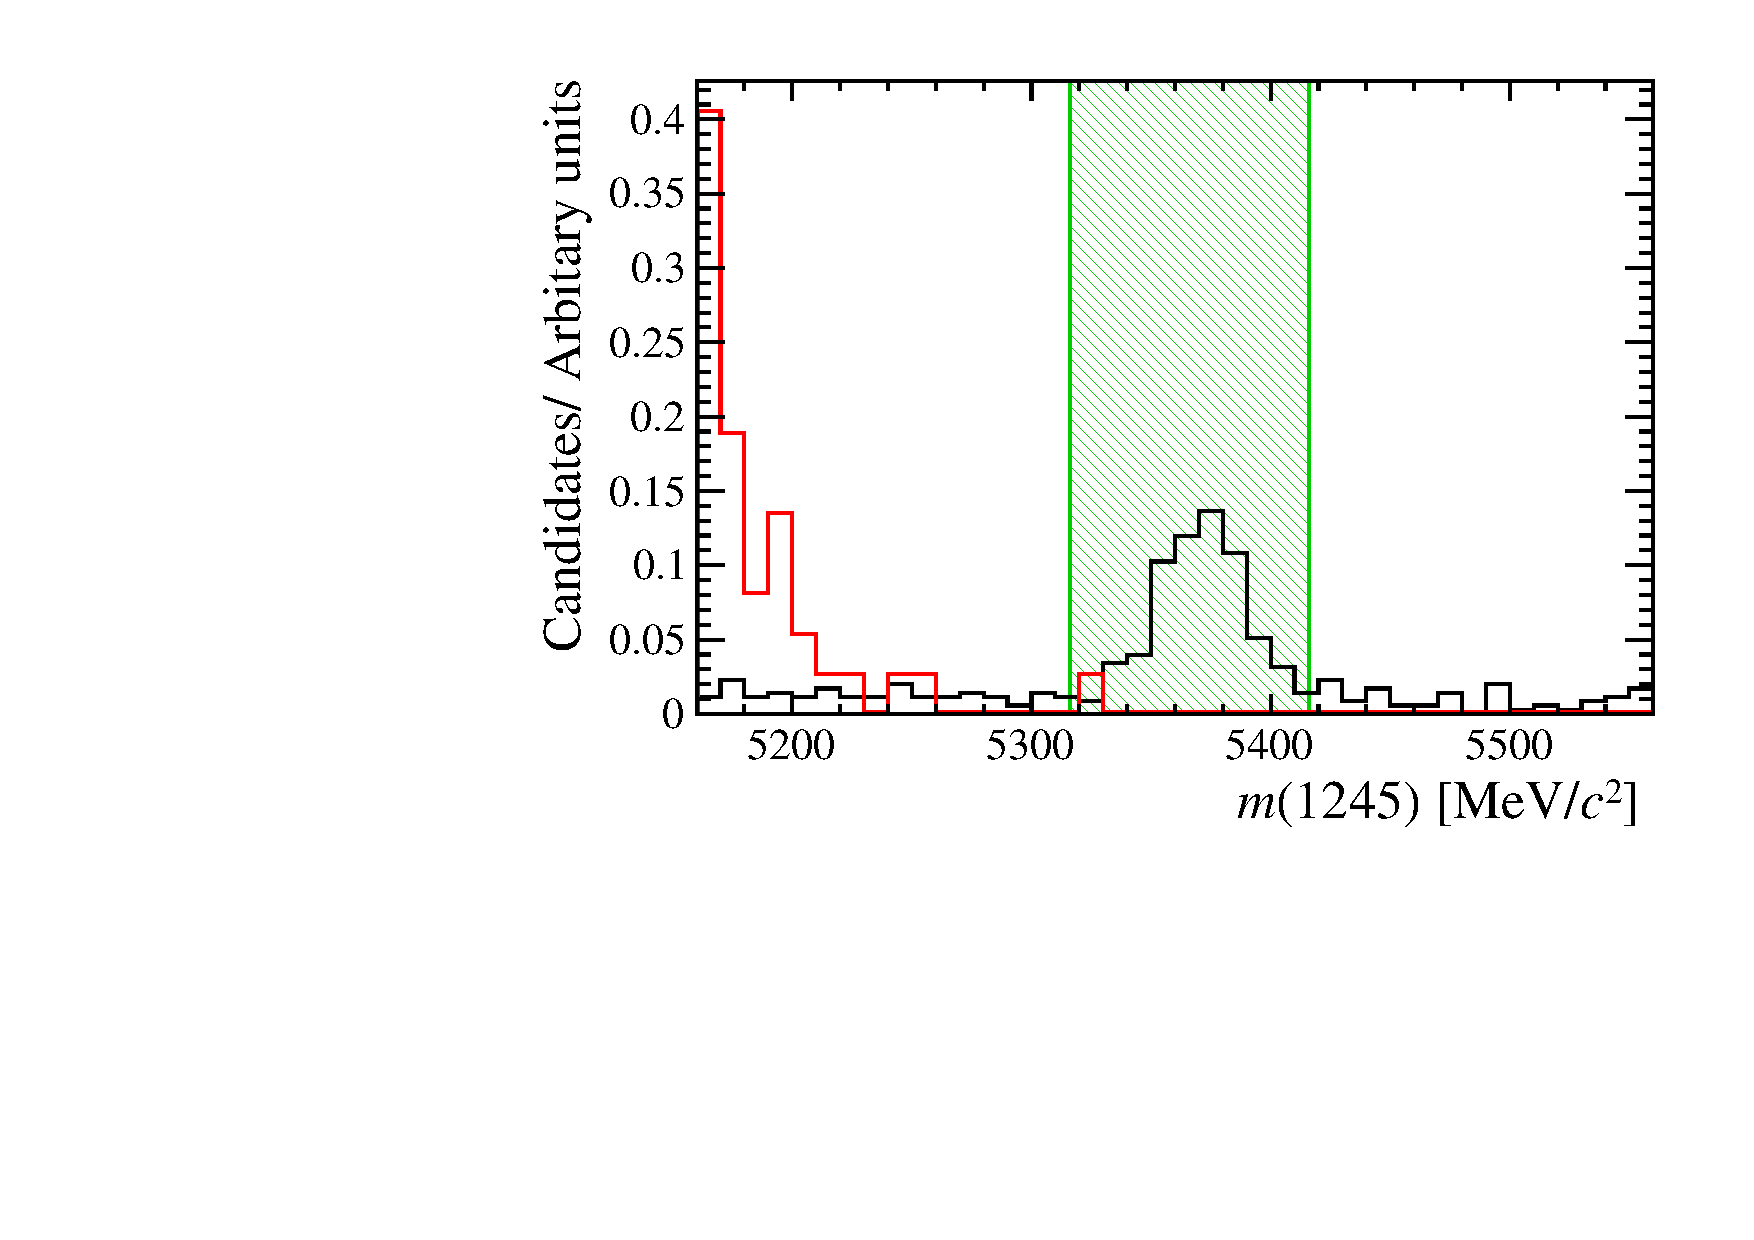
\includegraphics[width=1.0\textwidth]{figs/Selection/Veto_Comparison_B2DsPhi_Ds2KKPi_m1245.pdf}
      \end{subfigure}
      \begin{subfigure}[t]{0.32\textwidth}
         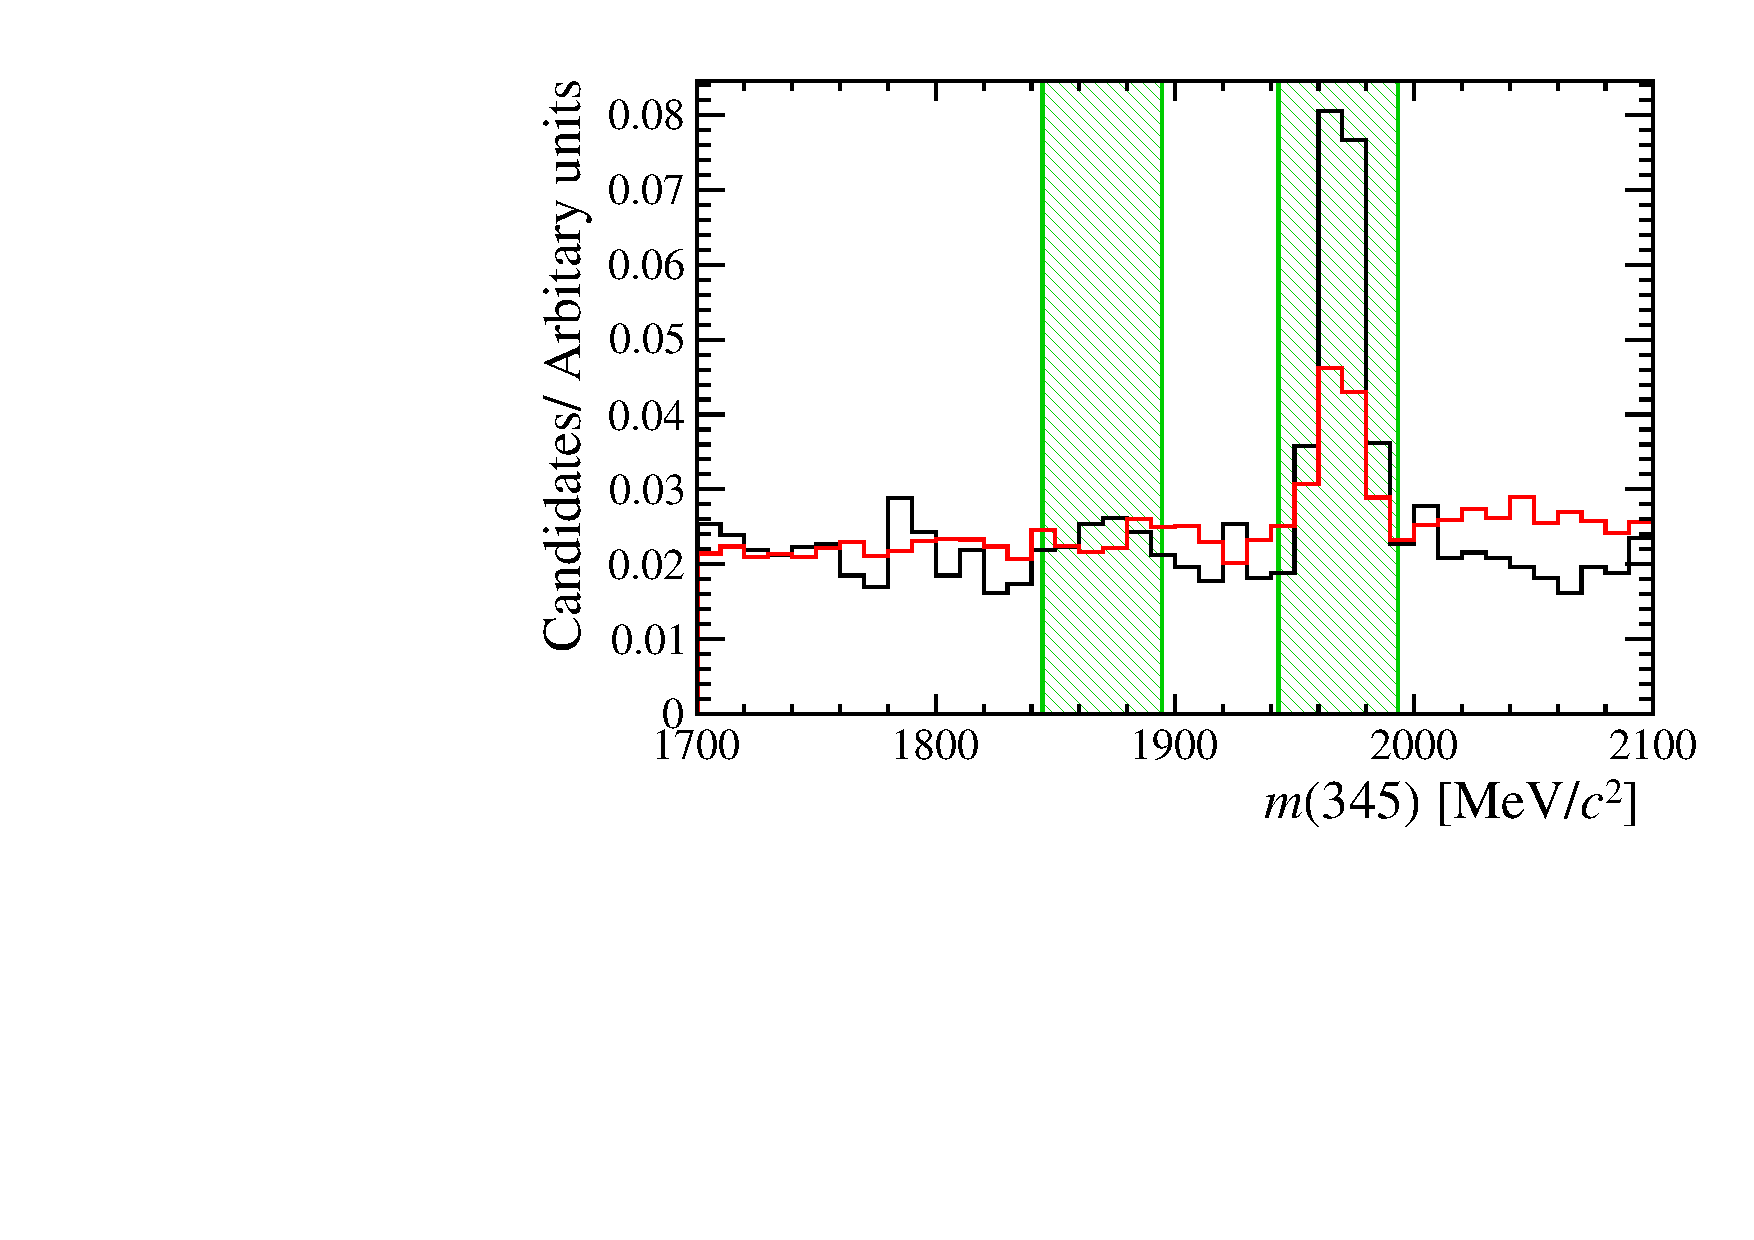
\includegraphics[width=1.0\textwidth]{figs/Selection/Veto_Comparison_B2DsPhi_Ds2KKPi_m345.pdf}
      \end{subfigure}
      \caption{\decay{\Bp}{(\decay{\Dsp}{\Kp\Km\pip})\phiz}}
   \end{subfigure}
   \begin{subfigure}[t]{1.0\textwidth}
      \centering
      \begin{subfigure}[t]{0.32\textwidth}
         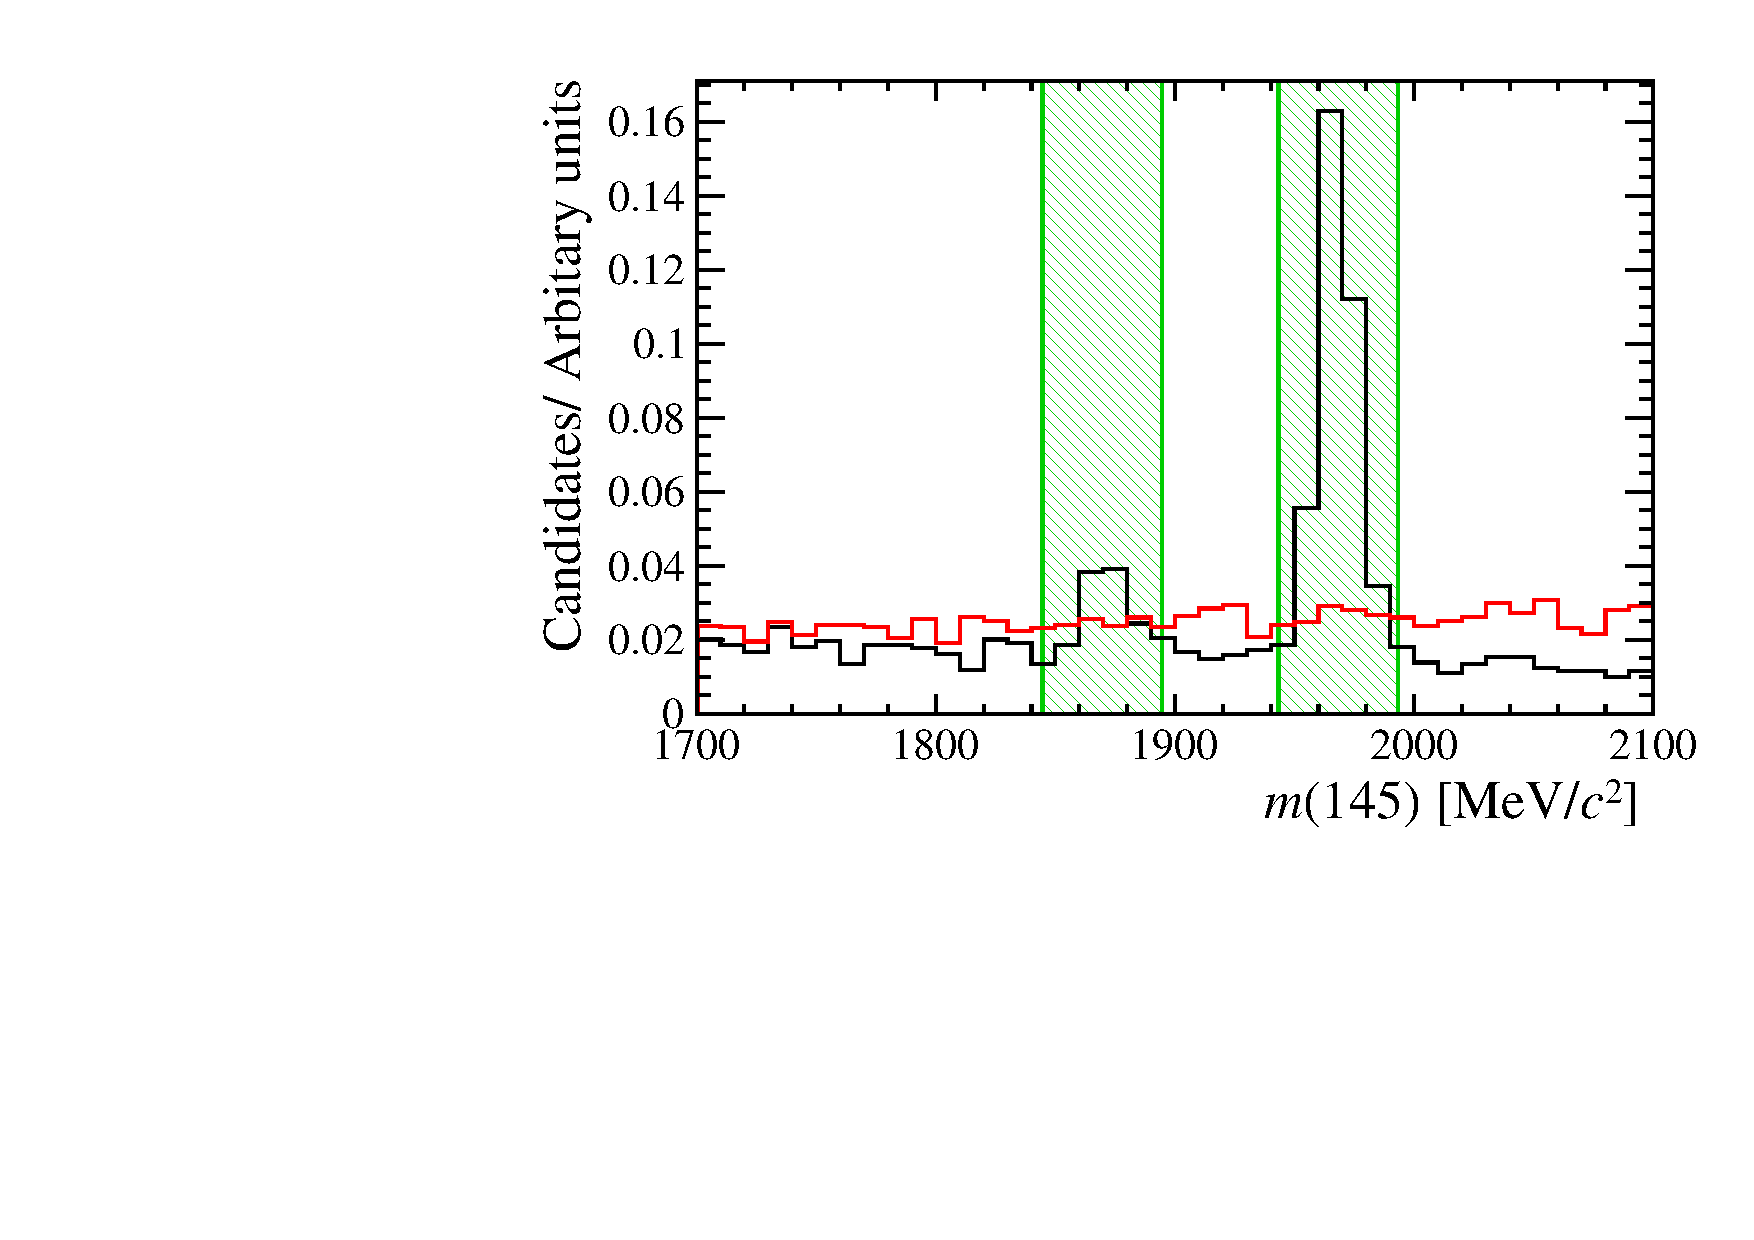
\includegraphics[width=1.0\textwidth]{figs/Selection/Veto_Comparison_B2DsPhi_Ds2PiPiPi_m145.pdf}
      \end{subfigure}
      \begin{subfigure}[t]{0.32\textwidth}
         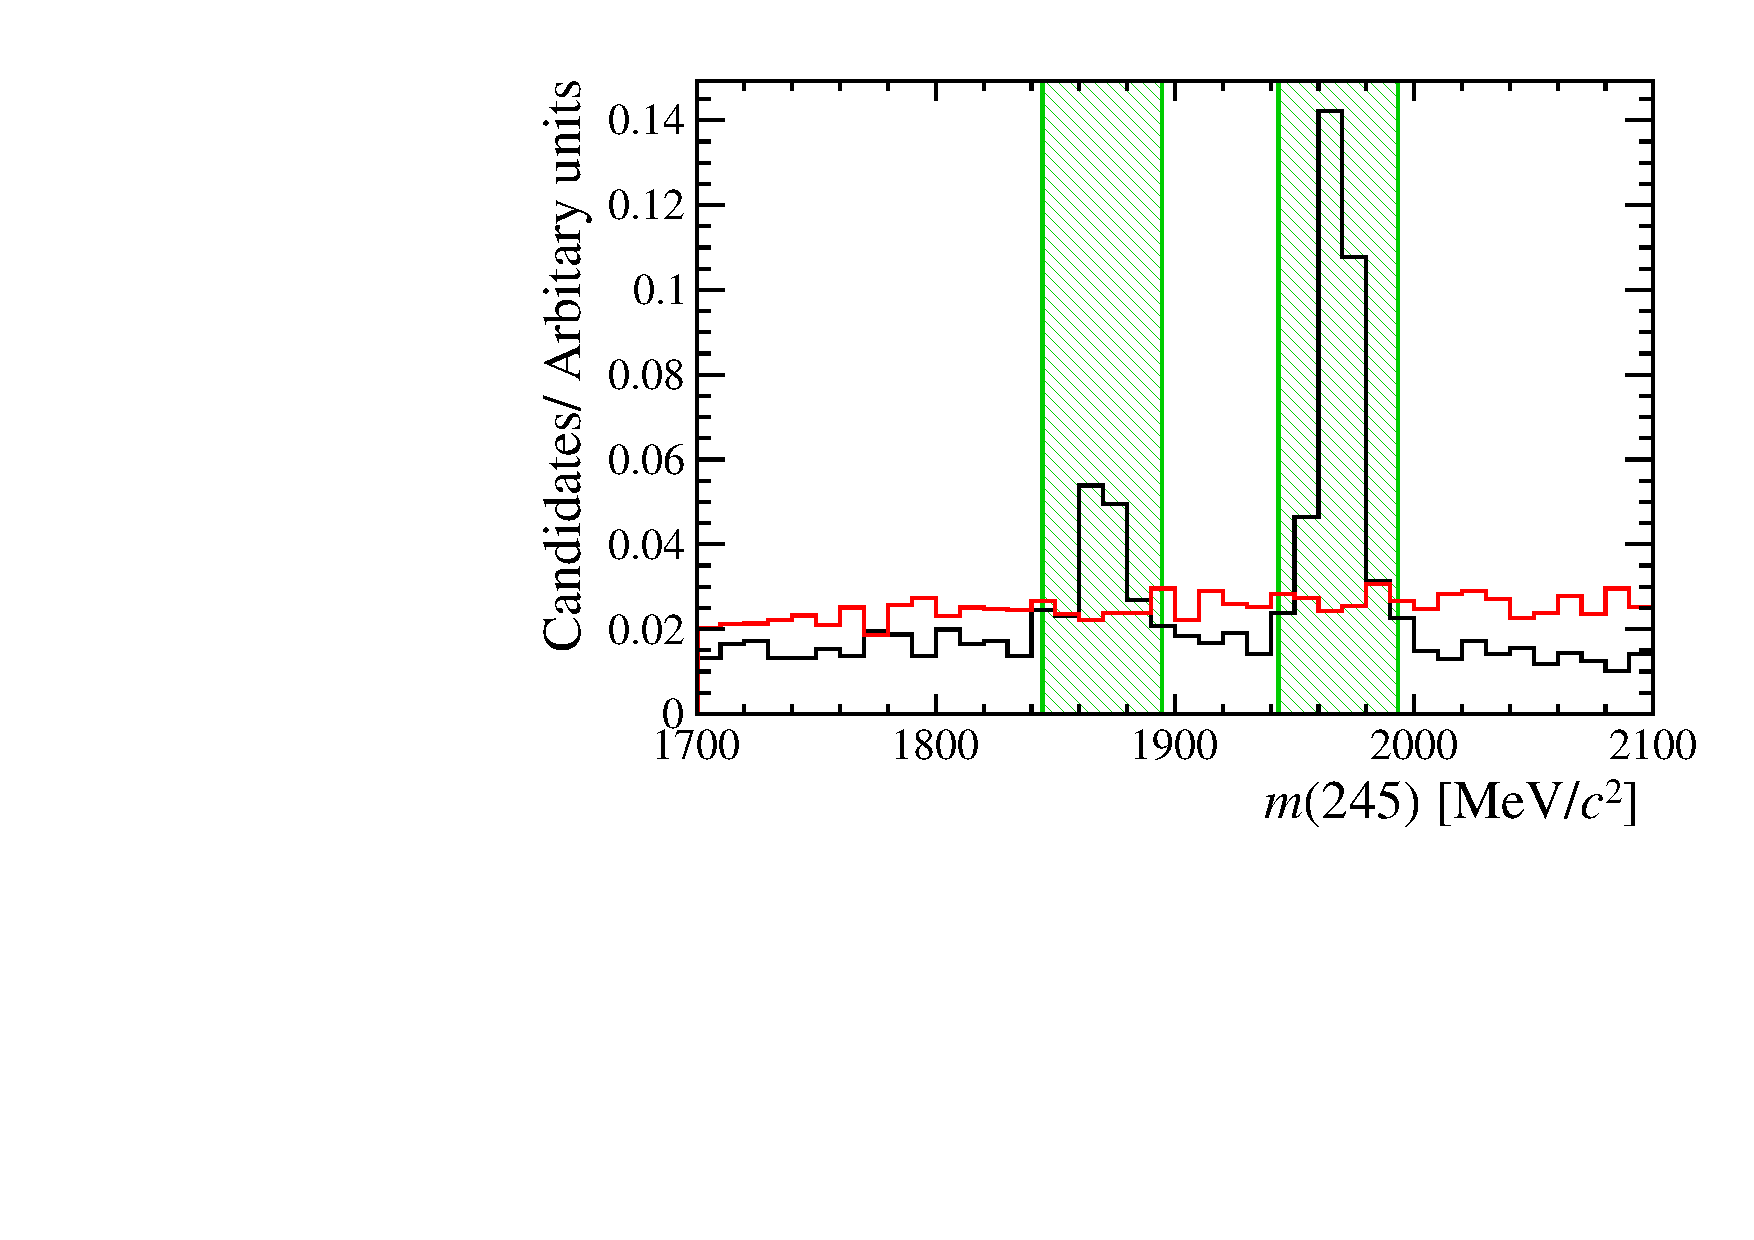
\includegraphics[width=1.0\textwidth]{figs/Selection/Veto_Comparison_B2DsPhi_Ds2PiPiPi_m245.pdf}
      \end{subfigure}
      \begin{subfigure}[t]{0.32\textwidth}
         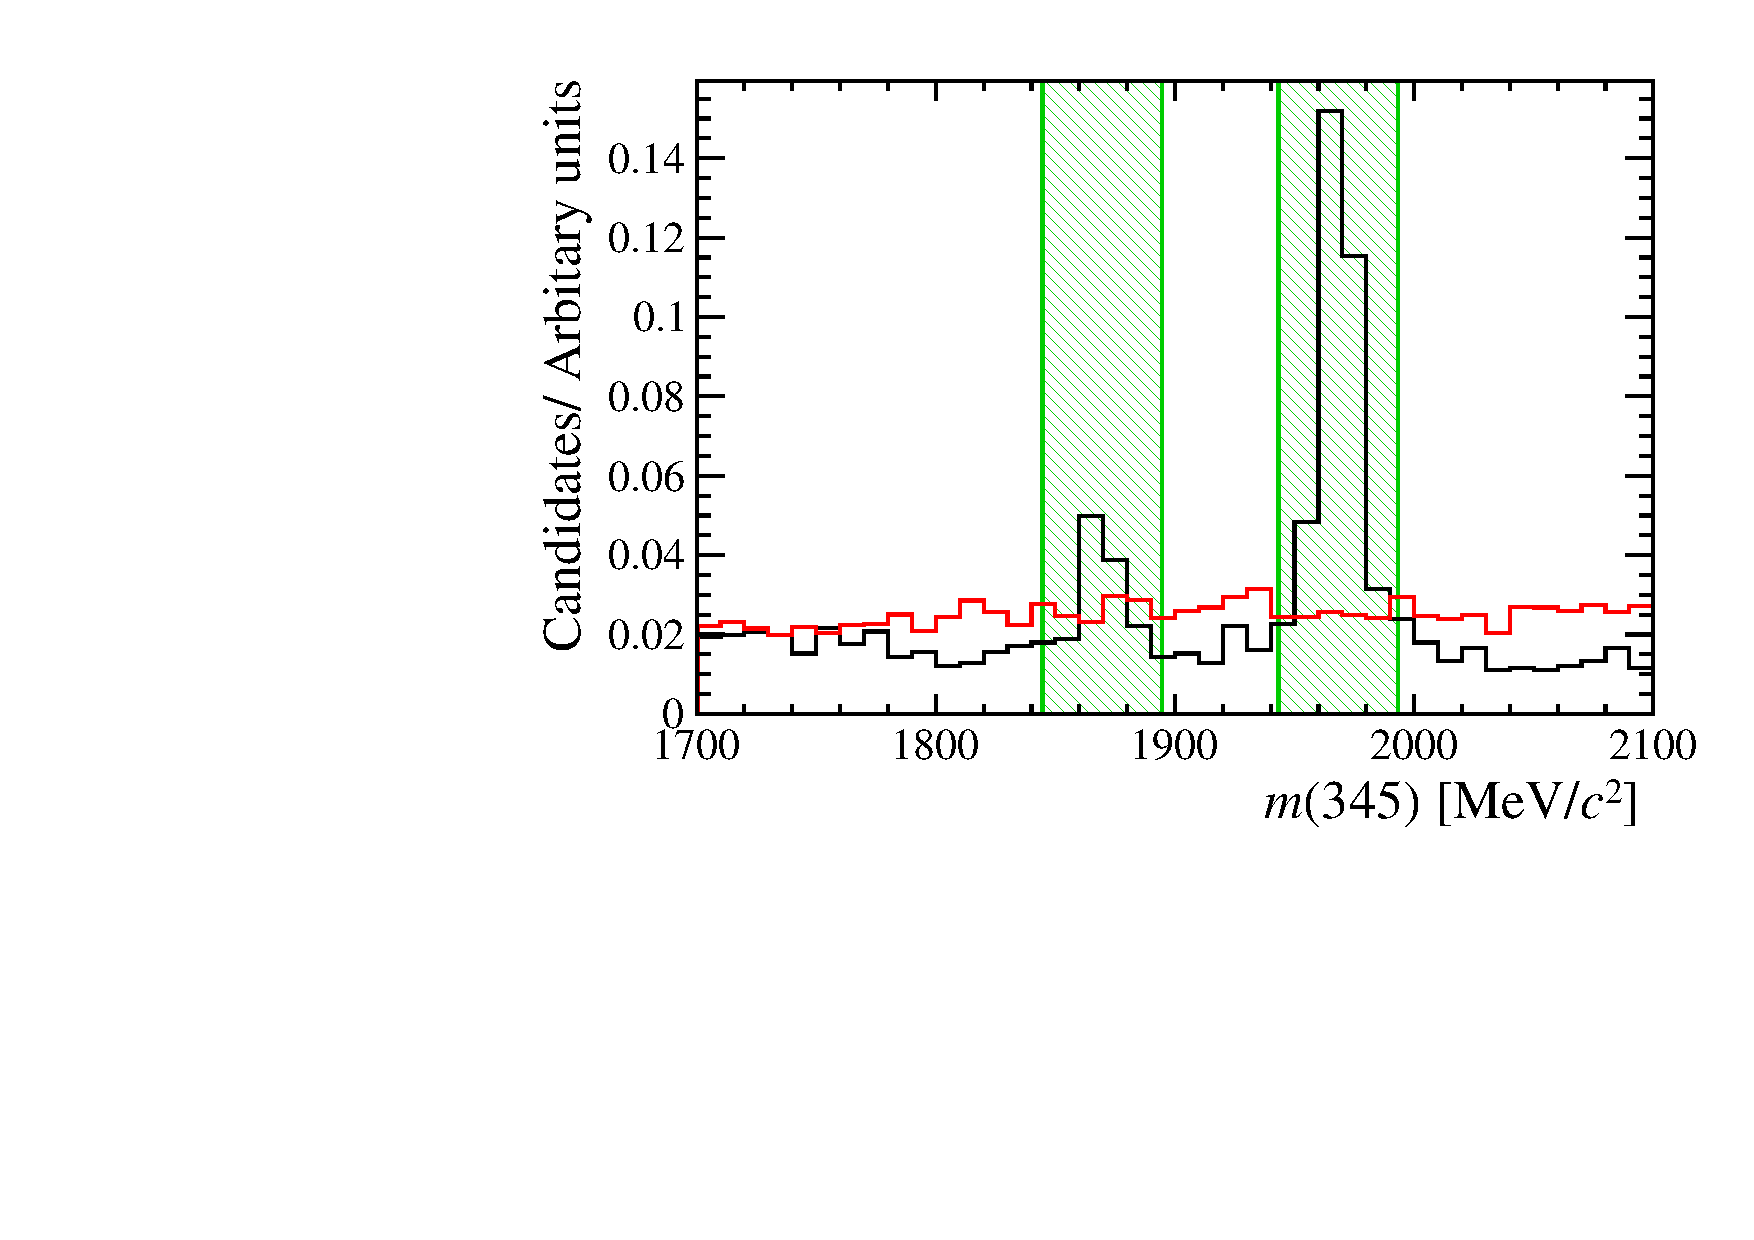
\includegraphics[width=1.0\textwidth]{figs/Selection/Veto_Comparison_B2DsPhi_Ds2PiPiPi_m345.pdf}
      \end{subfigure}
      \caption{\decay{\Bp}{(\decay{\Dsp}{\pip\pim\pip})\phiz}}
   \end{subfigure}
   \begin{subfigure}[t]{1.0\textwidth}
      \centering
      \begin{subfigure}[t]{0.32\textwidth}
         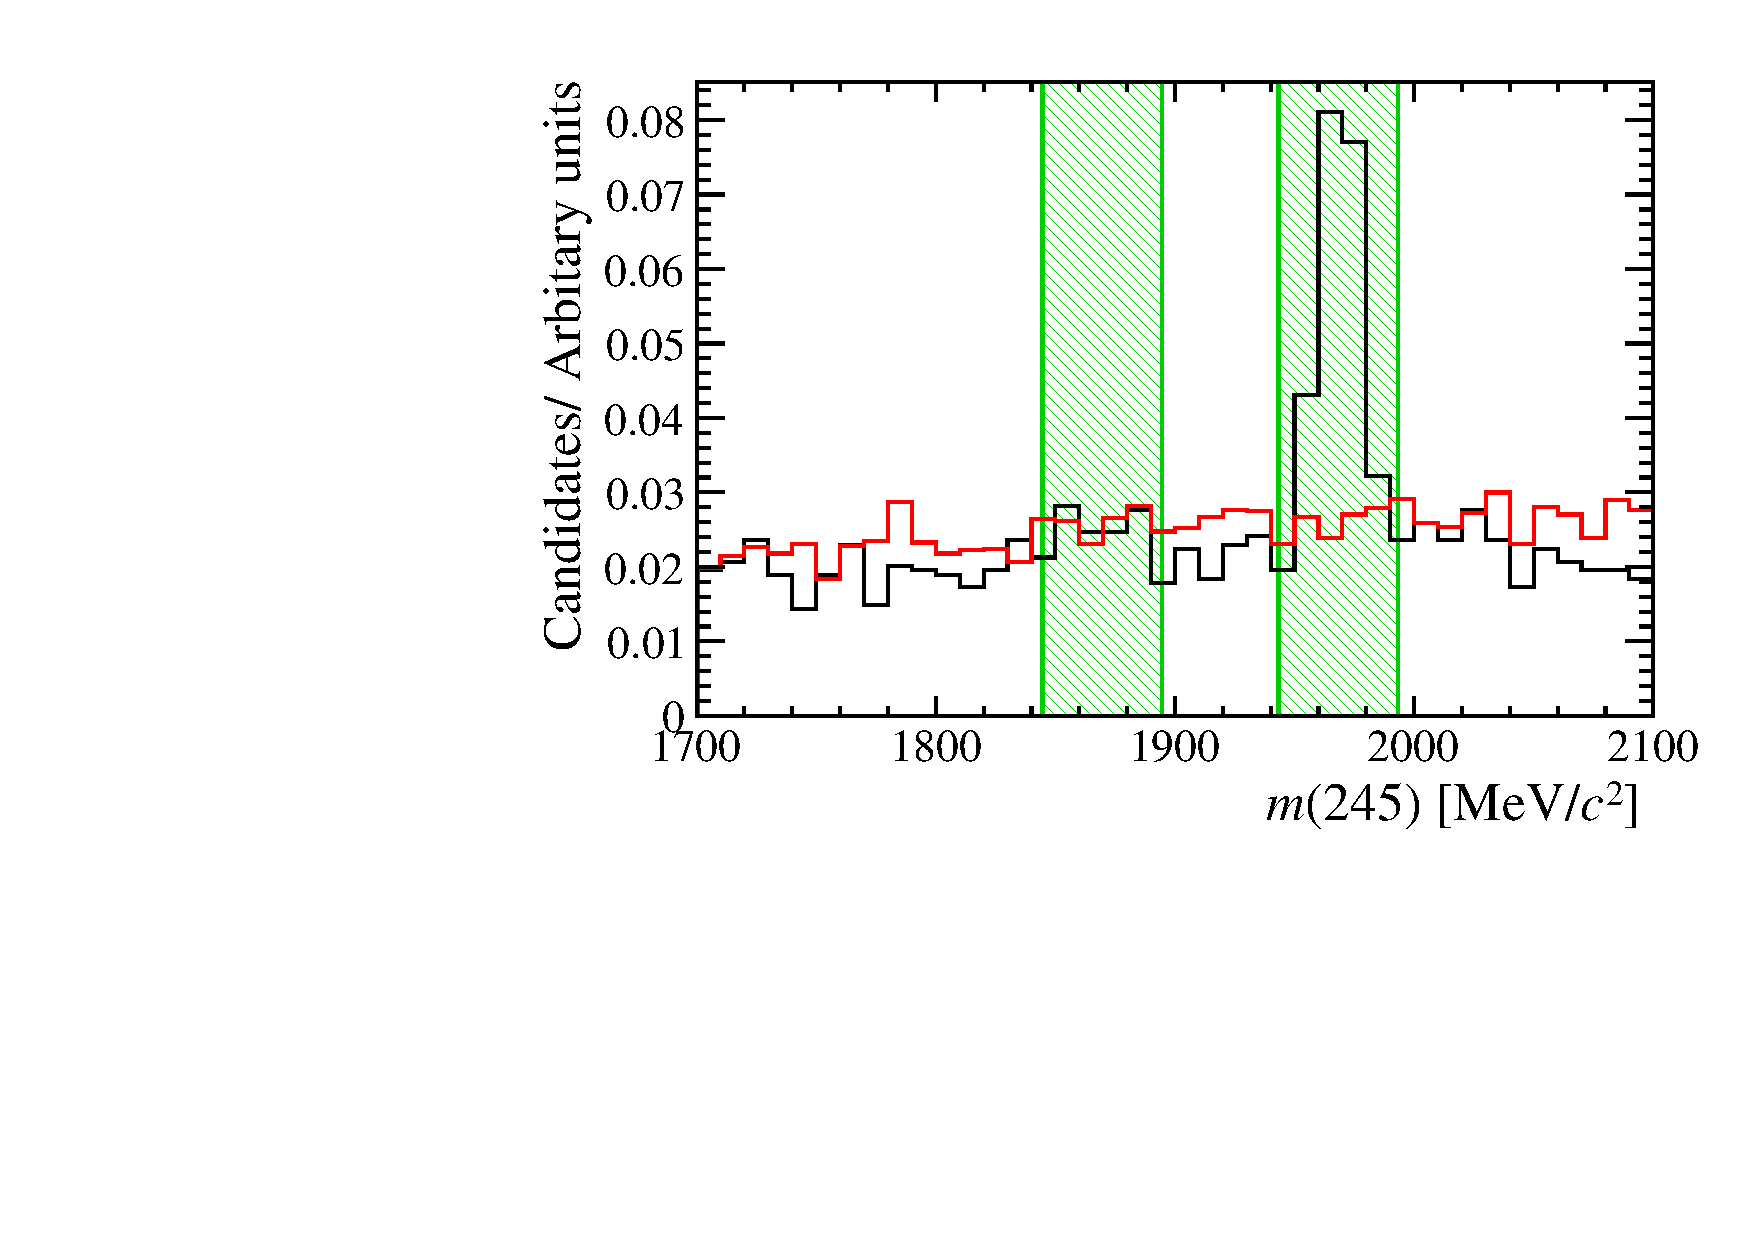
\includegraphics[width=1.0\textwidth]{figs/Selection/Veto_Comparison_B2DsPhi_Ds2KPiPi_m245.pdf}
      \end{subfigure}
      \begin{subfigure}[t]{0.32\textwidth}
         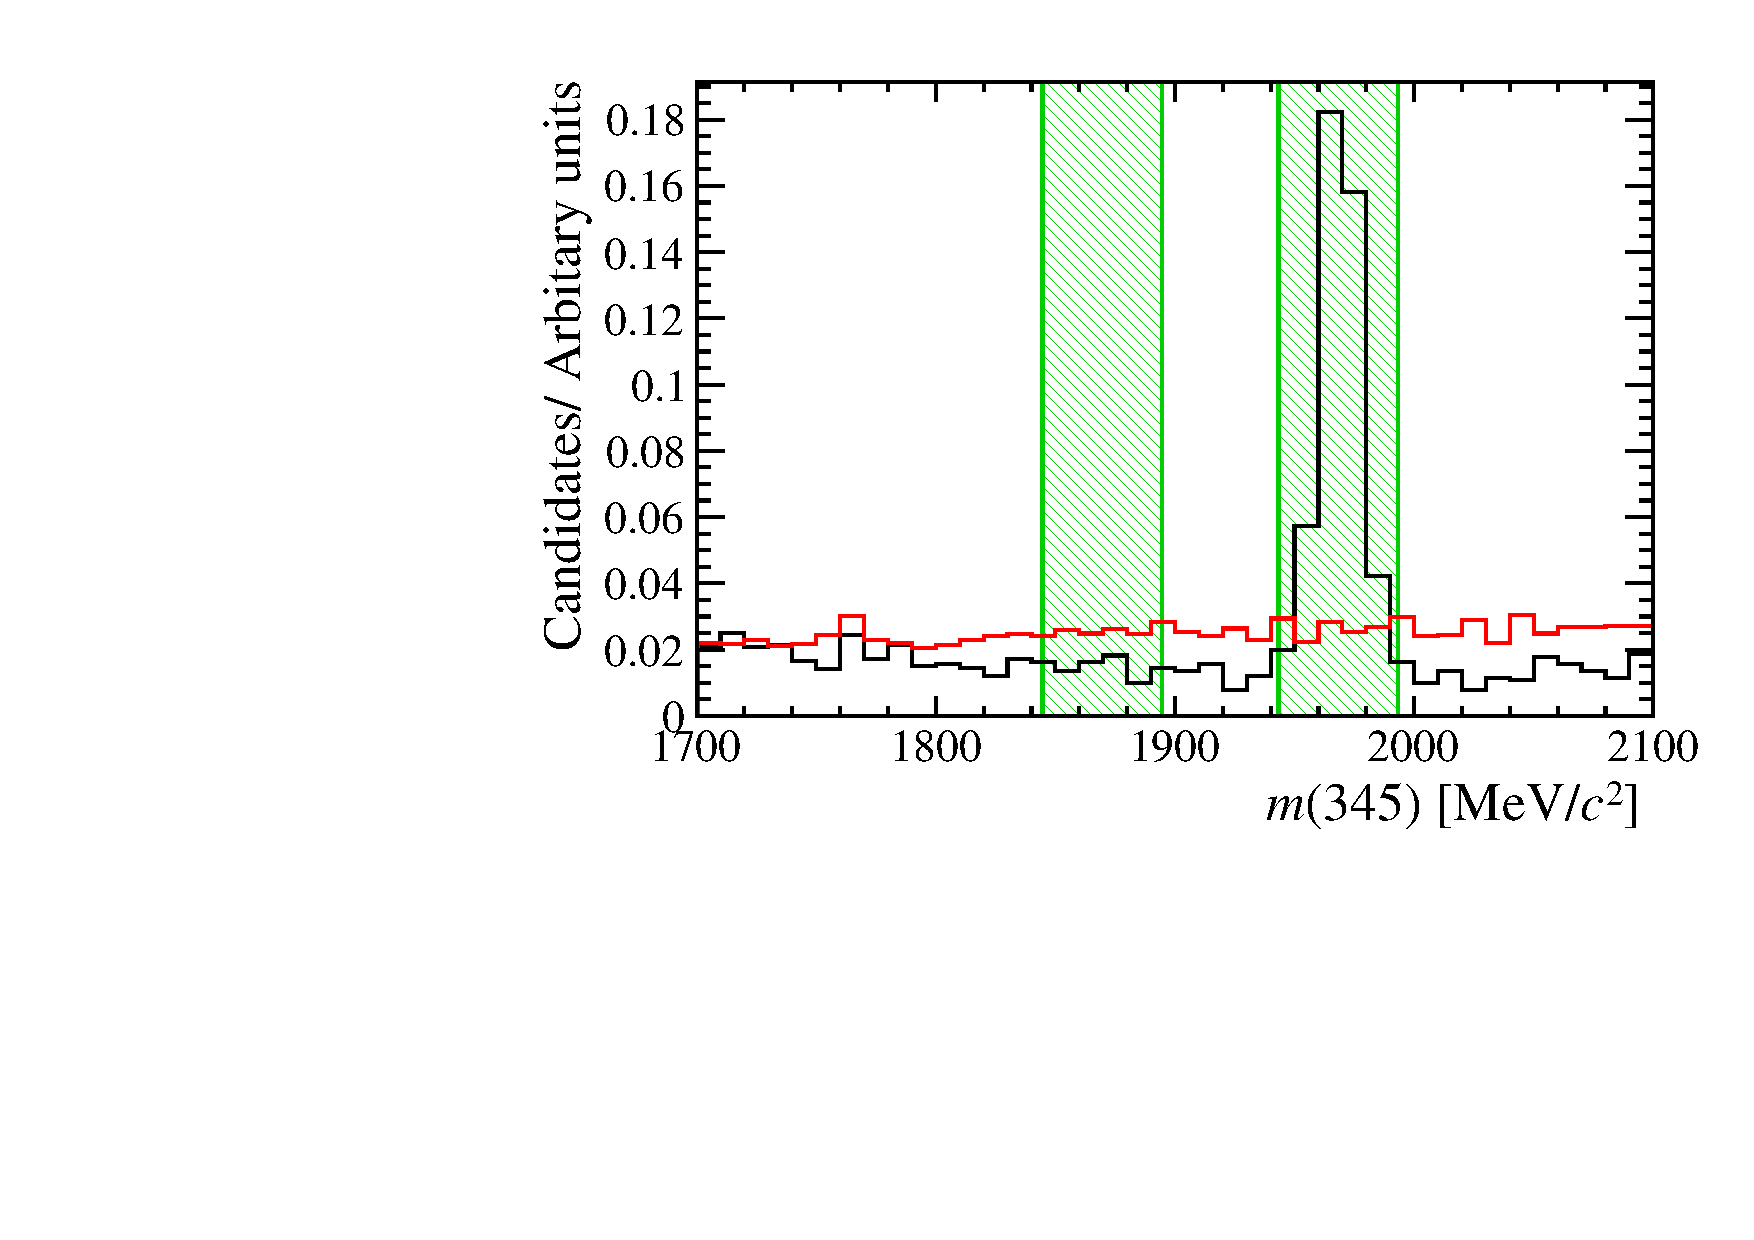
\includegraphics[width=1.0\textwidth]{figs/Selection/Veto_Comparison_B2DsPhi_Ds2KPiPi_m345.pdf}
      \end{subfigure}
      \caption{\decay{\Bp}{(\decay{\Dsp}{\Kp\pim\pip})\phiz}}
   \end{subfigure}

   \caption{Invariant mass distributions for subsets of decay products in data (black) and simulation (red). The green region show the regions removed by the vetoes listed in Sec~\ref{sec:kinematicvetos}.}
   \label{fig:invariantmassvetoes}   
\end{figure}
%%%%%%%%%%%%%%%%%%%%%%%%%%%%%%%%%%%%%%%%%%%%%%%%%%%%%%%%%%


In the search for \decay{\Bp}{\Dsp\Kp\Km} decays the increased size of the $m(\Kp\Km)$ phase-space means more of the combinations of final state particles are susceptible to sharp peaking structure from incorrectly reconstructed backgrounds. Those spectra found to have significant peaking structures are additionally vetoed, as shown in Fig.~\ref{fig:invariantmassvetoes_DsKK}.

\begin{itemize}
\item Vetoes for the mode \decay{\Bp}{(\decay{\Dsp}{\Kp\Km\pip})\Kp\Km}:
\begin{itemize}
\item $|m(\text{1245})- m(\Bs)| > 50\mevcc$
\item $|m(\text{345})- m(\Dsp)| > 25\mevcc$ and $|m(\text{345})- m(\Dp)| > 25\mevcc$
\item $|m(\text{135})- m(\Dsp)| > 25\mevcc$
\item $|m(\text{234})- m(\Dsp)| > 25\mevcc$
\end{itemize}
\end{itemize}

%%%%%%%%%%%%%%%%%%%%%%%%%%%%%%%%%%%%%%%%%%%%%%%%%%%%%%%%%%
\begin{figure}[!h]
   \centering
   \begin{subfigure}[t]{1.0\textwidth}
      \centering
      \begin{subfigure}[t]{0.32\textwidth}
         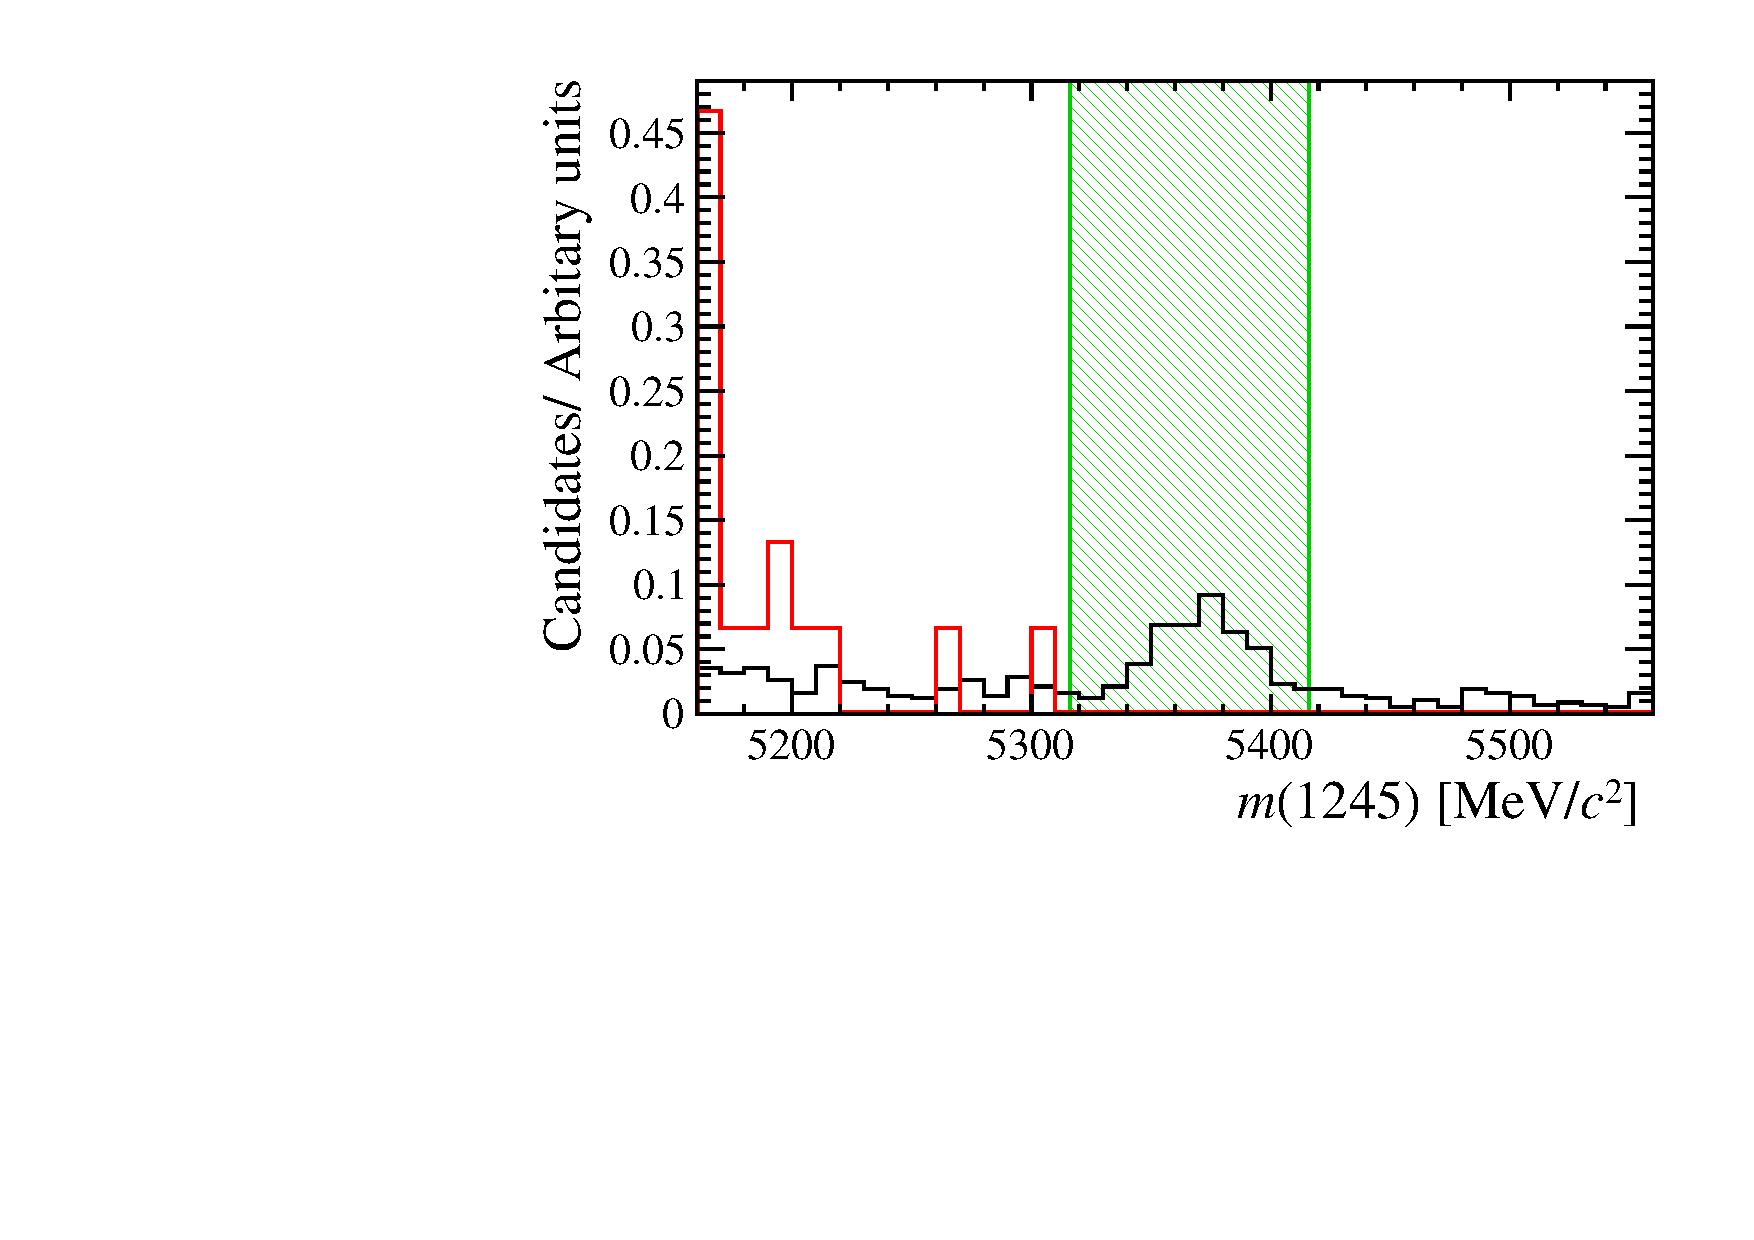
\includegraphics[width=1.0\textwidth]{figs/Selection/Veto_Comparison_B2DsKK_Ds2KKPi_m1245.pdf}
      \end{subfigure}\\
      \begin{subfigure}[t]{0.32\textwidth}
         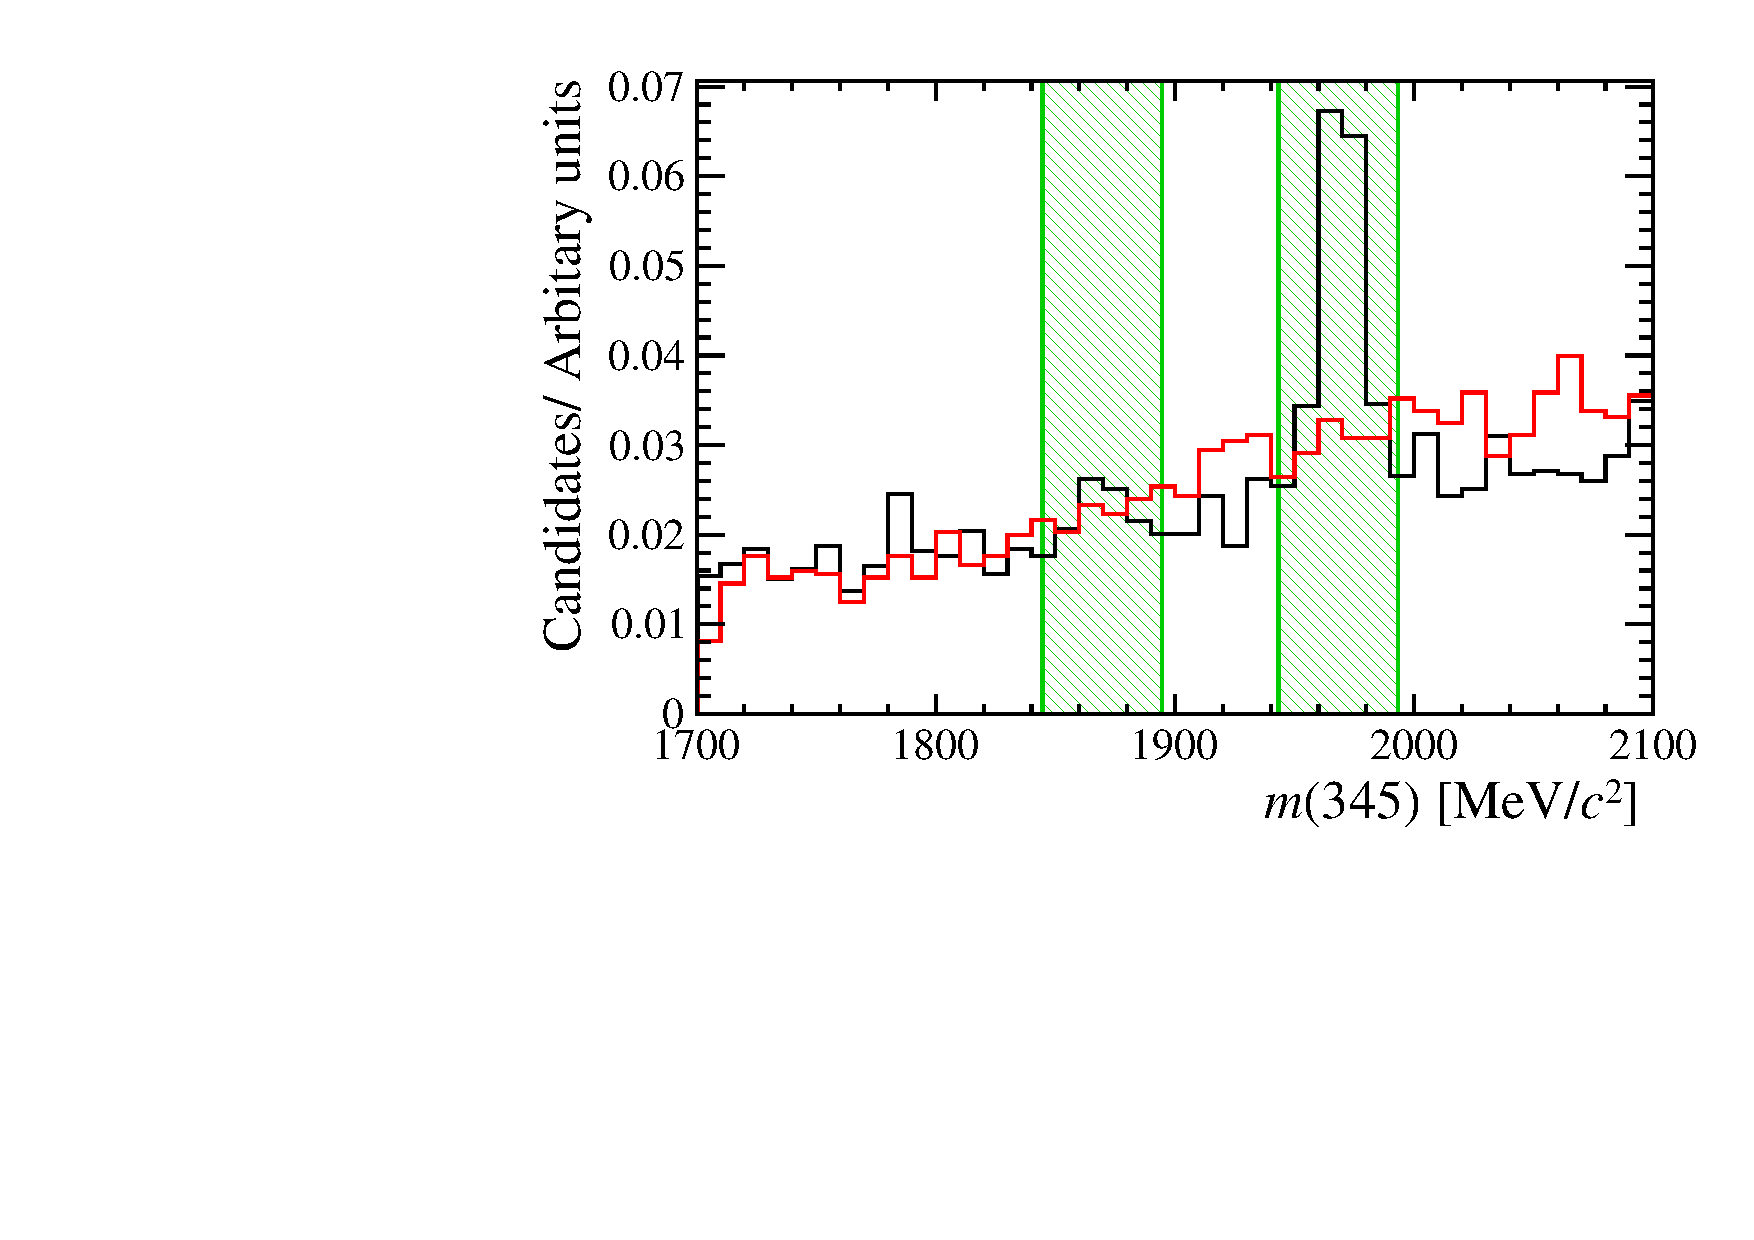
\includegraphics[width=1.0\textwidth]{figs/Selection/Veto_Comparison_B2DsKK_Ds2KKPi_m345.pdf}
      \end{subfigure}
      \begin{subfigure}[t]{0.32\textwidth}
         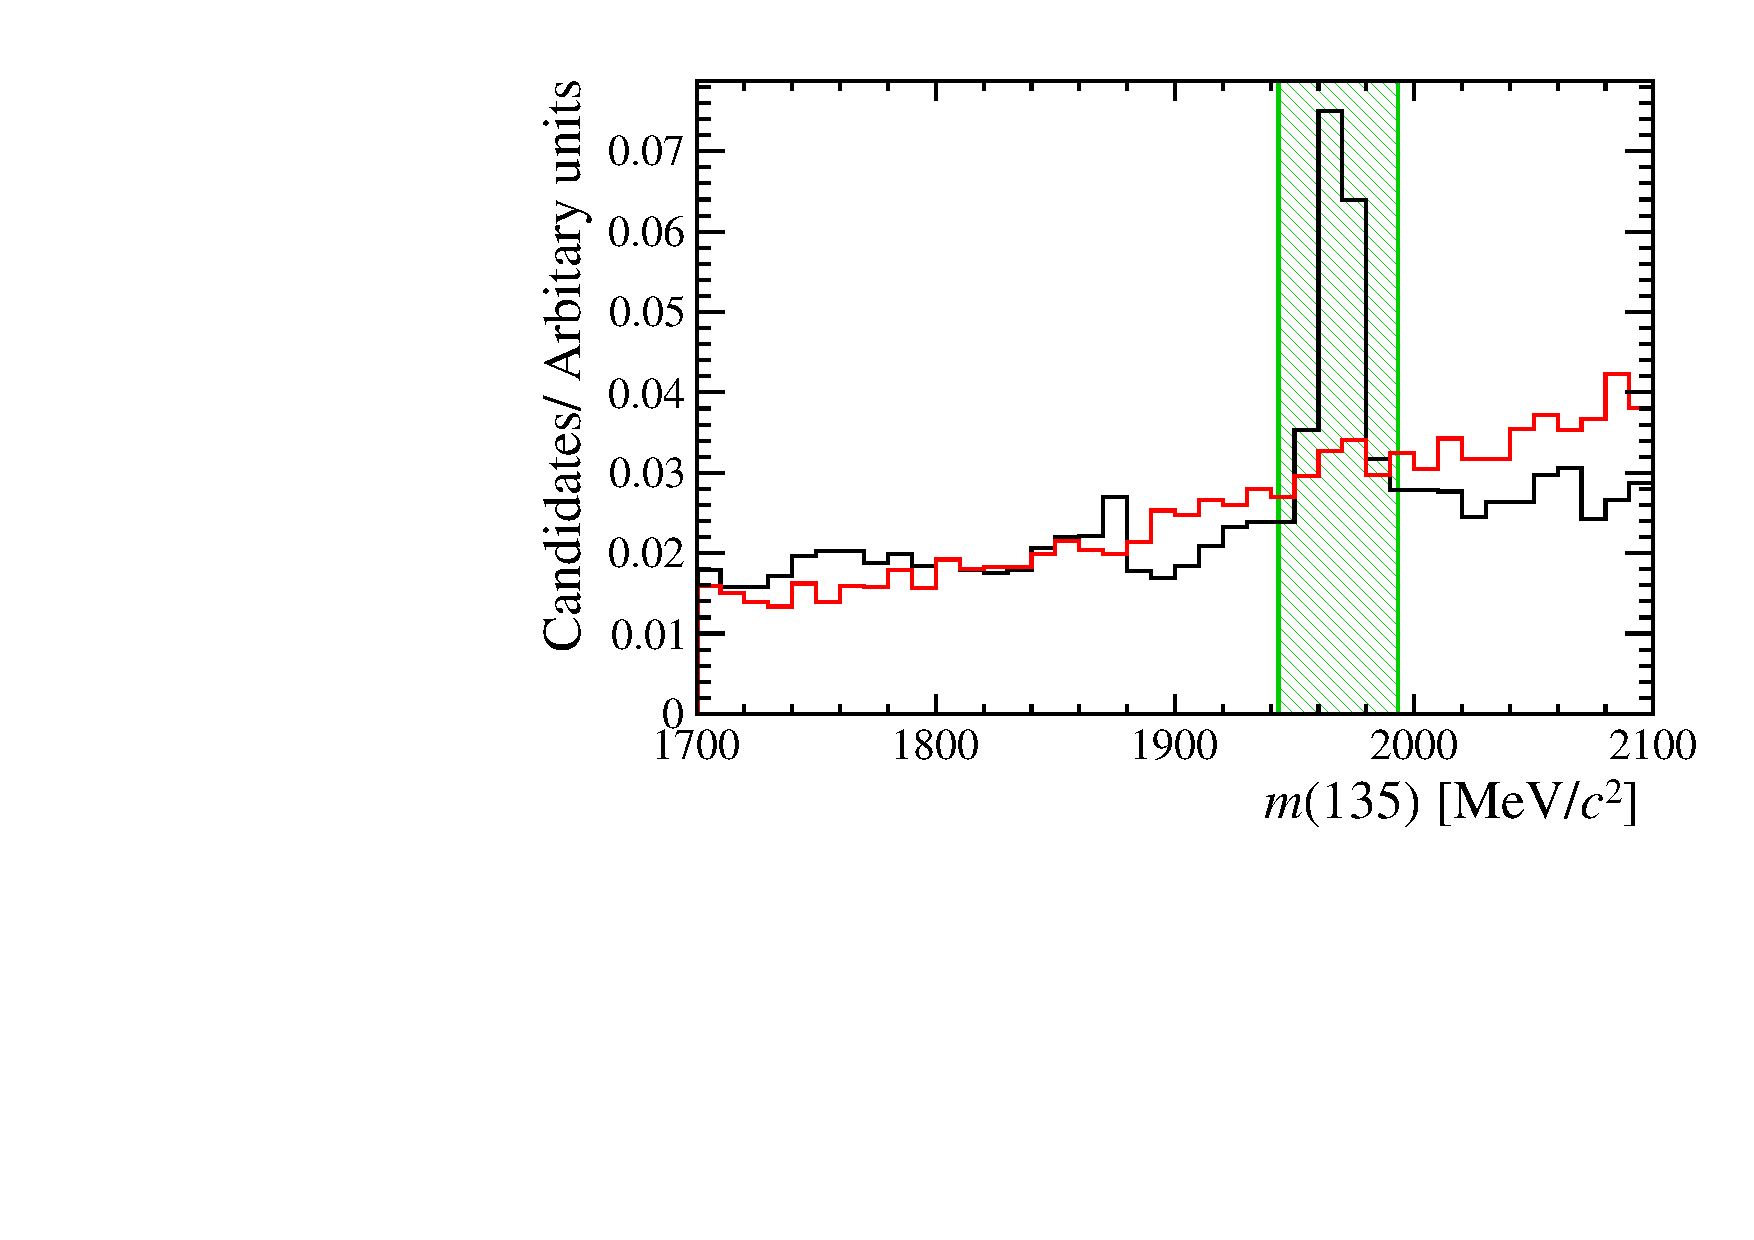
\includegraphics[width=1.0\textwidth]{figs/Selection/Veto_Comparison_B2DsKK_Ds2KKPi_m135.pdf}
      \end{subfigure}
      \begin{subfigure}[t]{0.32\textwidth}
         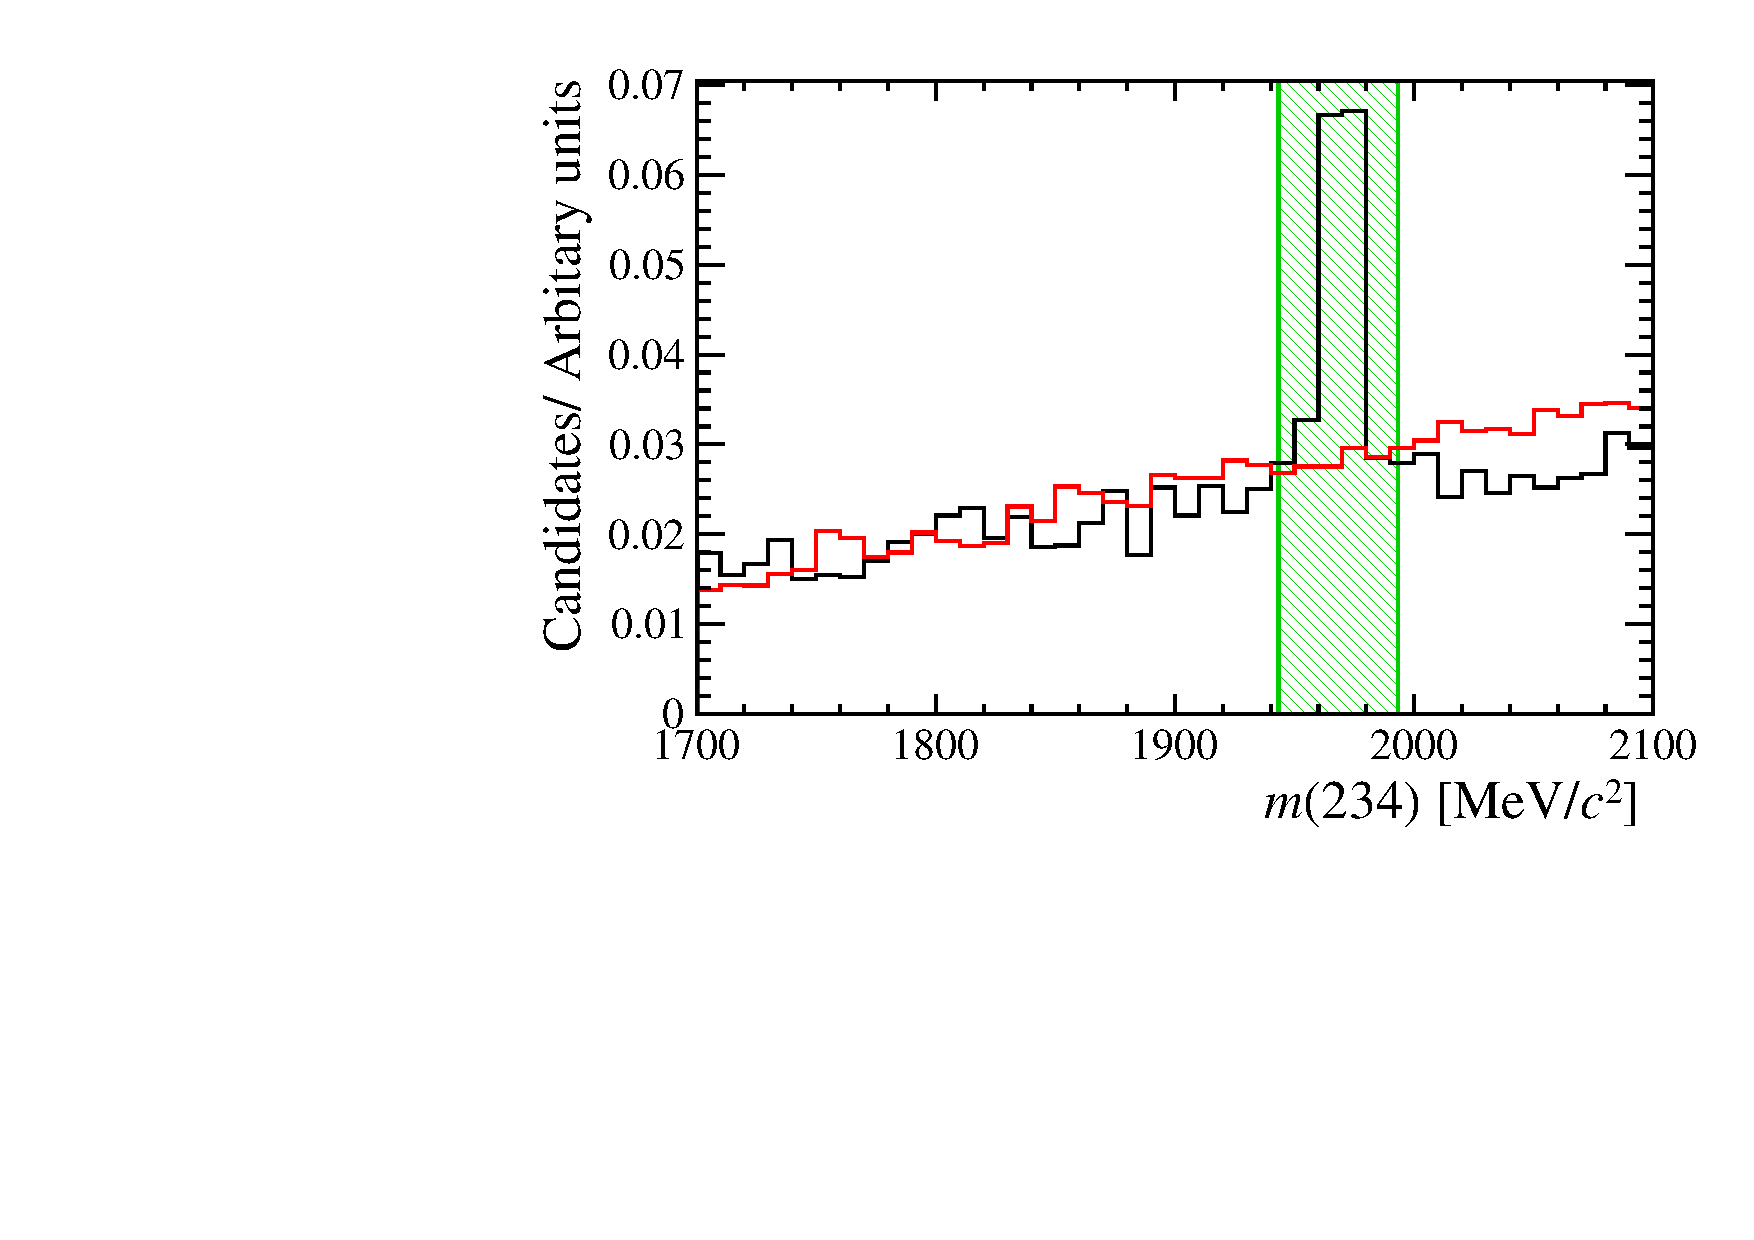
\includegraphics[width=1.0\textwidth]{figs/Selection/Veto_Comparison_B2DsKK_Ds2KKPi_m234.pdf}
      \end{subfigure}
   \end{subfigure}

   \caption{Invariant mass distributions for subsets of decay products for \decay{\Bp}{(\decay{\Dsp}{\Kp\Km\pip})\Kp\Km} decays in data (black) and simulation (red). The green region show the regions removed by the vetoes listed in Sec~\ref{sec:kinematicvetos}.}
   \label{fig:invariantmassvetoes_DsKK}   
\end{figure}
%%%%%%%%%%%%%%%%%%%%%%%%%%%%%%%%%%%%%%%%%%%%%%%%%%%%%%%%%%

\section{Impact parameter requirements}
\label{sec:app_sel_IPchi2}

Requirements are placed on the impact parameter significance for the signal decays. The \Bp meson candidate is required to be consistent with originating at the PV by requiring $\chi^2_{\text{IP}} < 10$. This helps to remove background as unrelated combinations of \Dsp and \phiz mesons will not necessarily point back towards the PV.
Additionally, the opposite requirement is made of the \Dsp meson, $\chi^2_{\text{IP}} > 10$, to reduce charm meson backgrounds where the charm is produced promptly at the PV.


%%%%%%%%%%%%%%%%%%%%%%%%%%%%%%%%%%%%%%%%%%%%%%%%%%%%%%%%%%
\begin{figure}[!h]
   \centering
   \begin{subfigure}[t]{0.32\textwidth}
      \centering
      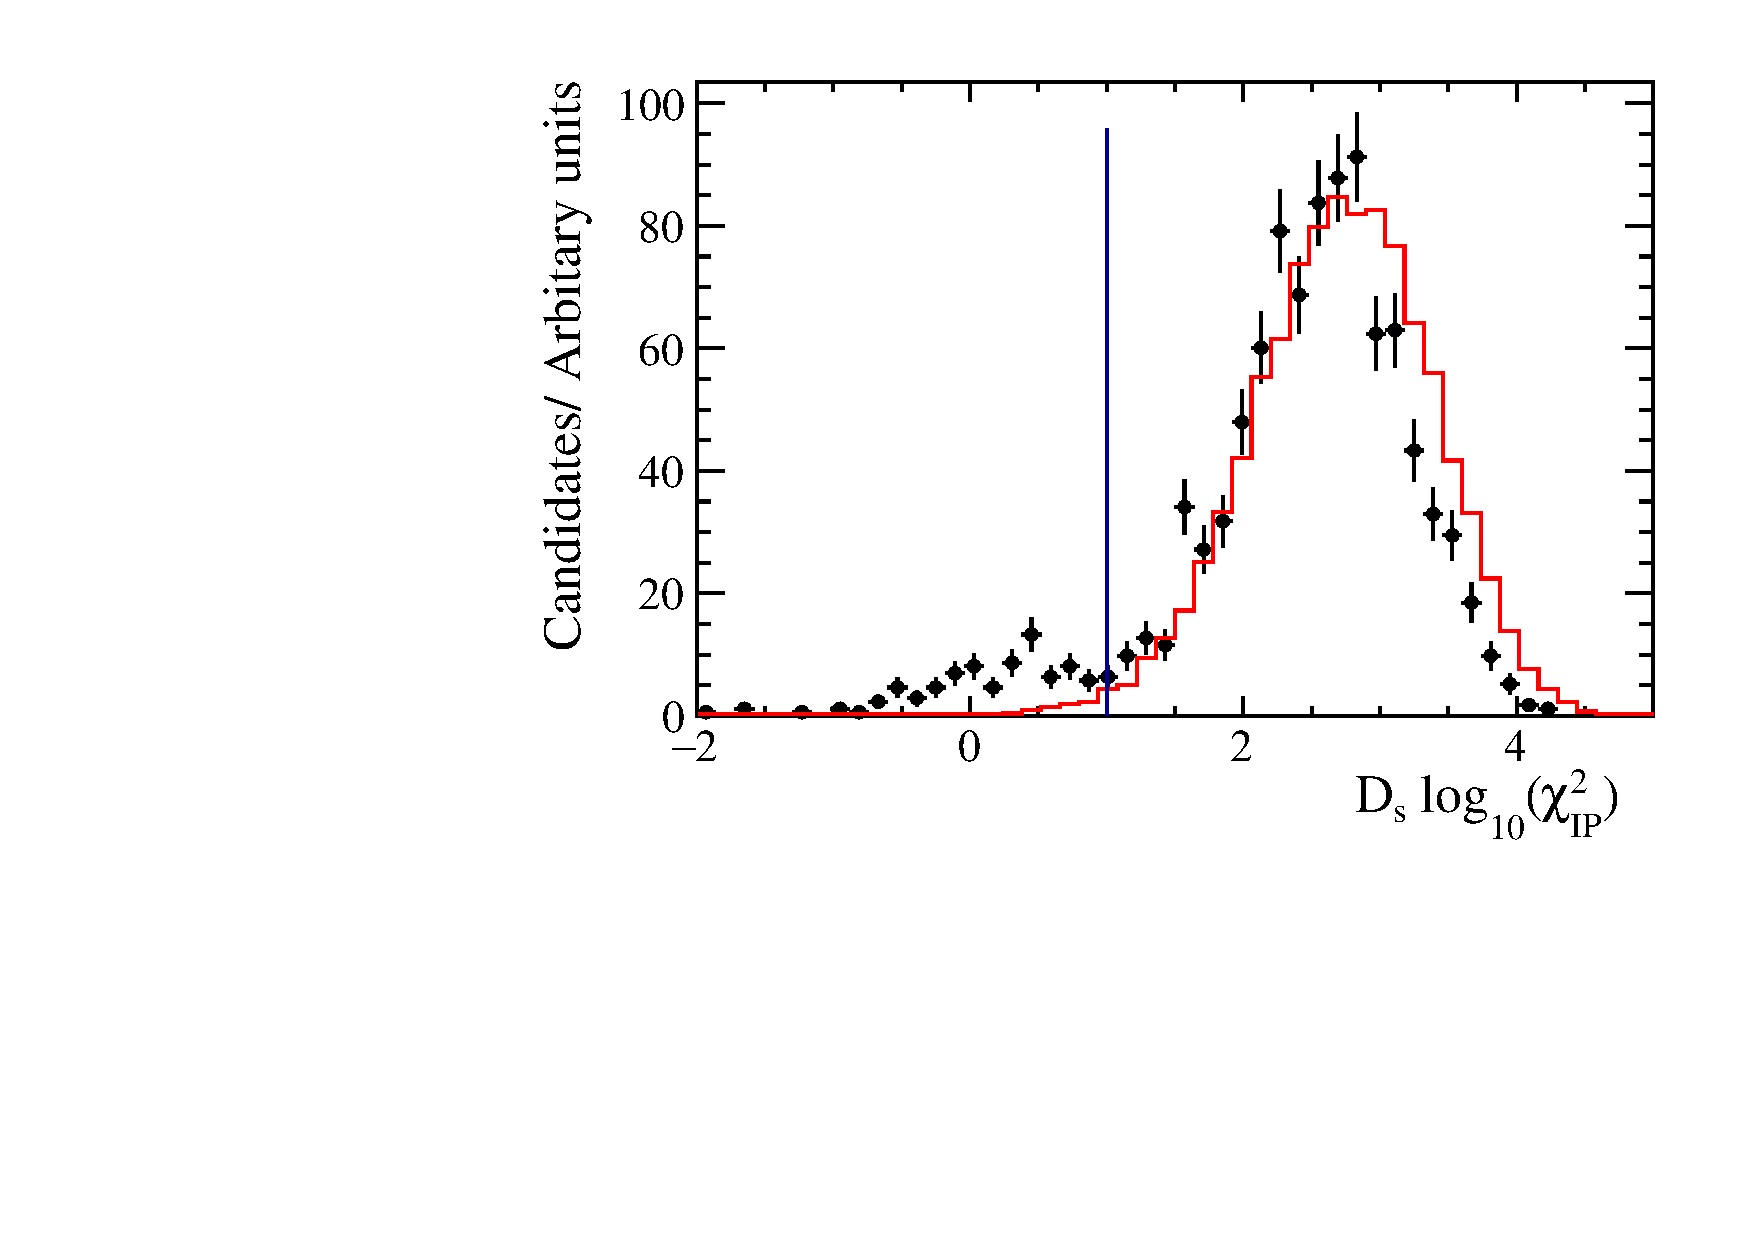
\includegraphics[width=1.0\textwidth]{figs/Selection/Data_MC_Comparison_Var_2_B2DsPhi_Ds2KKPi.pdf}
      \caption{\decay{\Dsp}{\Kp\Km\pip}}
   \end{subfigure}
   \begin{subfigure}[t]{0.32\textwidth}
      \centering
      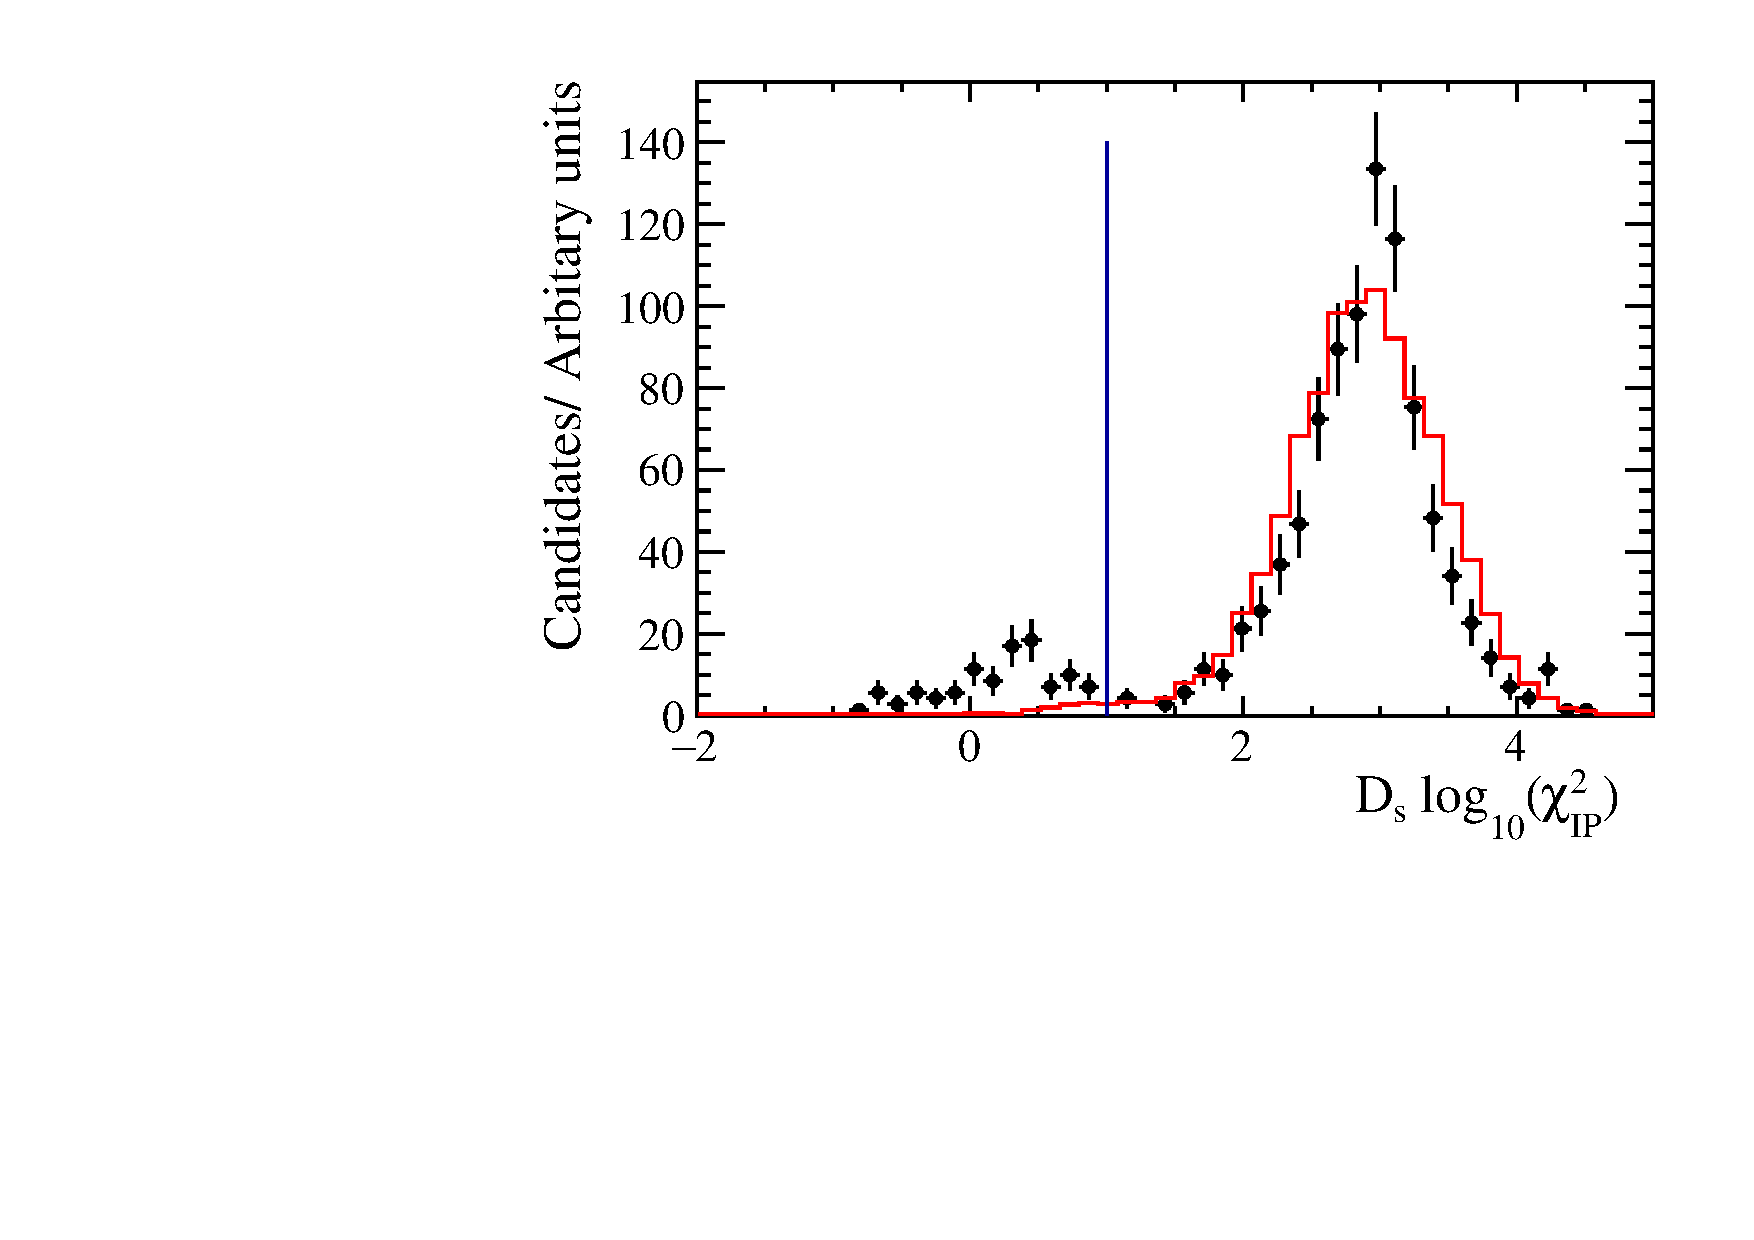
\includegraphics[width=1.0\textwidth]{figs/Selection/Data_MC_Comparison_Var_2_B2DsPhi_Ds2PiPiPi.pdf}
      \caption{\decay{\Dsp}{\pip\pim\pip}}
   \end{subfigure}
   \begin{subfigure}[t]{0.32\textwidth}
      \centering
      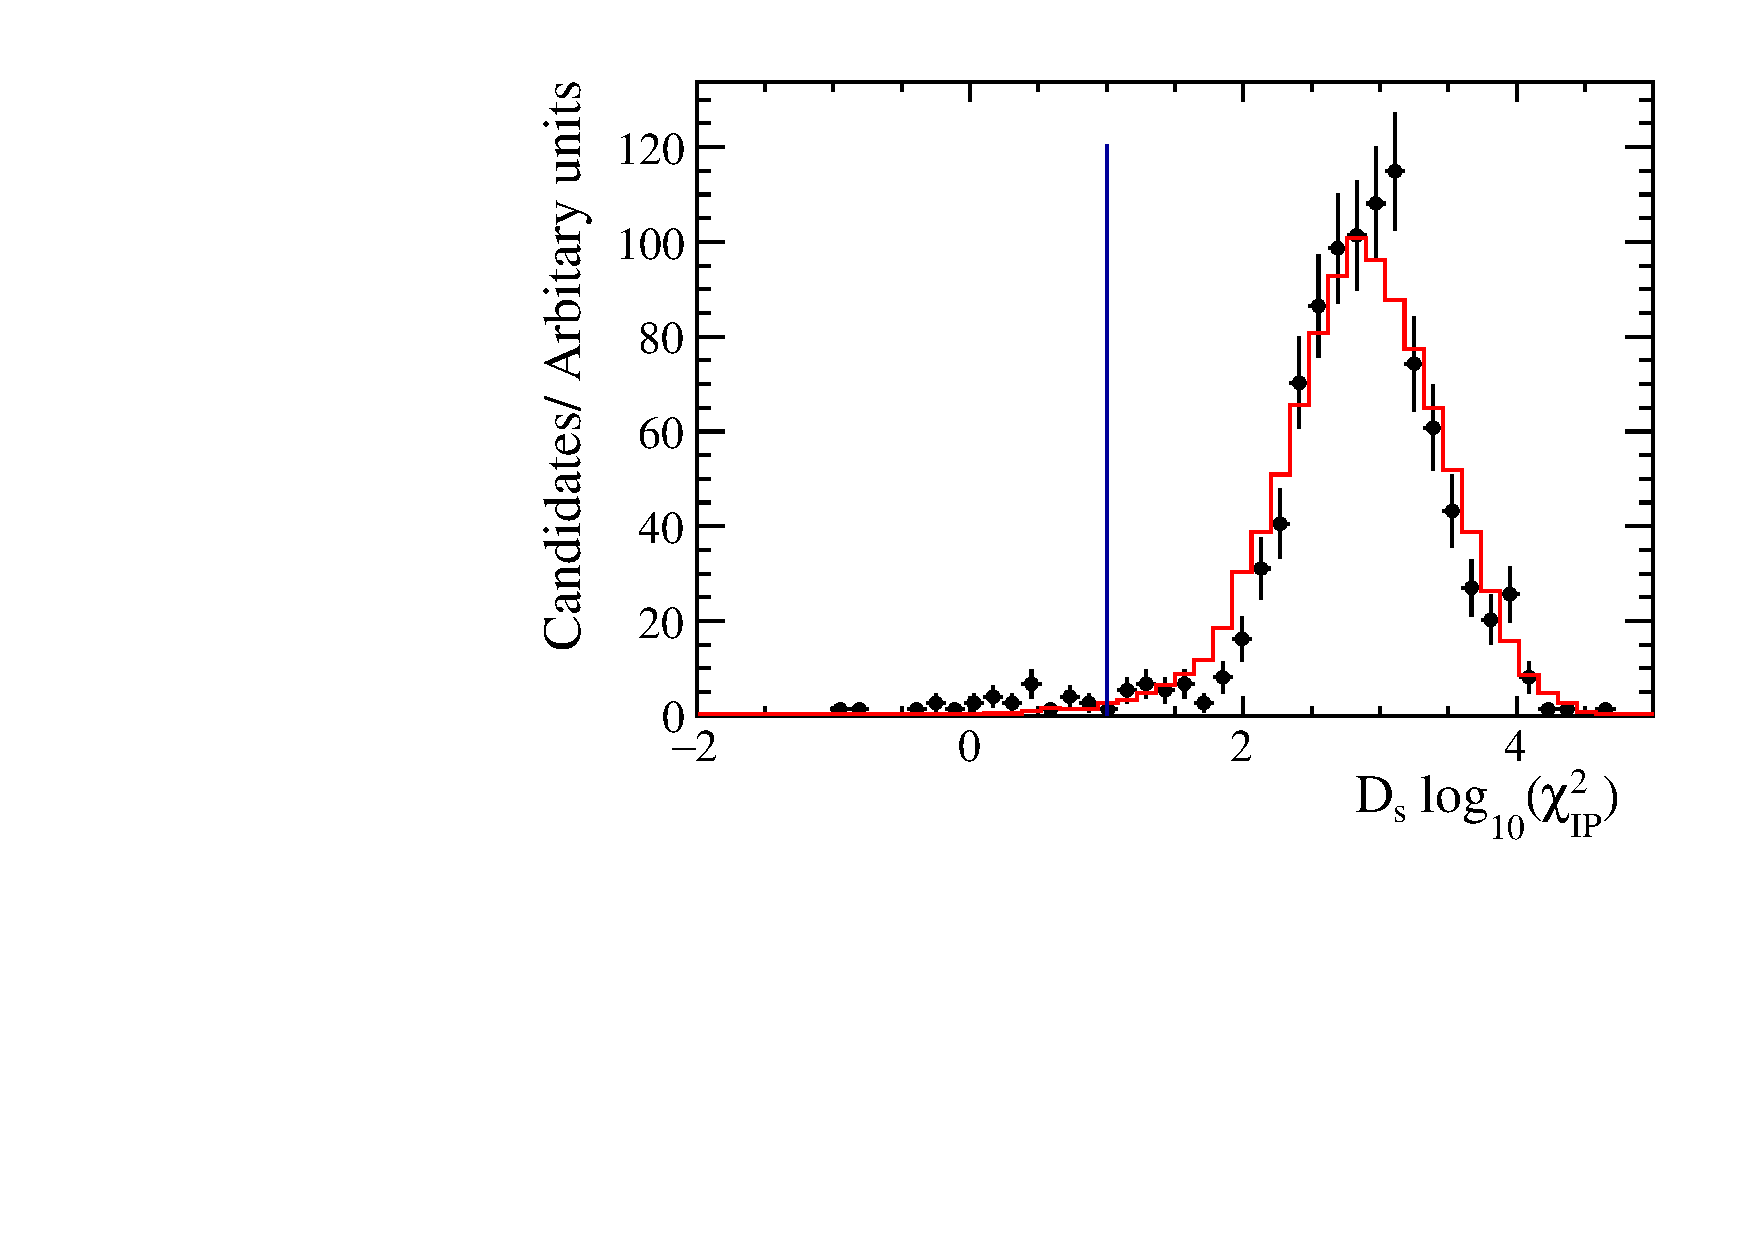
\includegraphics[width=1.0\textwidth]{figs/Selection/Data_MC_Comparison_Var_2_B2DsPhi_Ds2KPiPi.pdf}
      \caption{\decay{\Dsp}{\Kp\pim\pip}}
   \end{subfigure}\\
   \caption{The \Bp meson $\chi^{2}_{\text{IP}}$ distributions for \decay{\Bp}{\Dsp\phiz} candidates in data (black) and simulation (red) after the MVA selection. Candidates within the range $4900 < m(\Dsp\phiz) < 5900 \mevcc$ are included in these figures. Candidates to the left of the vertical line are retained.}
   \label{fig:ipchi2dist_signal_B}   
\end{figure}
%%%%%%%%%%%%%%%%%%%%%%%%%%%%%%%%%%%%%%%%%%%%%%%%%%%%%%%%%%

%%%%%%%%%%%%%%%%%%%%%%%%%%%%%%%%%%%%%%%%%%%%%%%%%%%%%%%%%%
\begin{figure}[!h]
   \centering
   \begin{subfigure}[t]{0.32\textwidth}
      \centering
      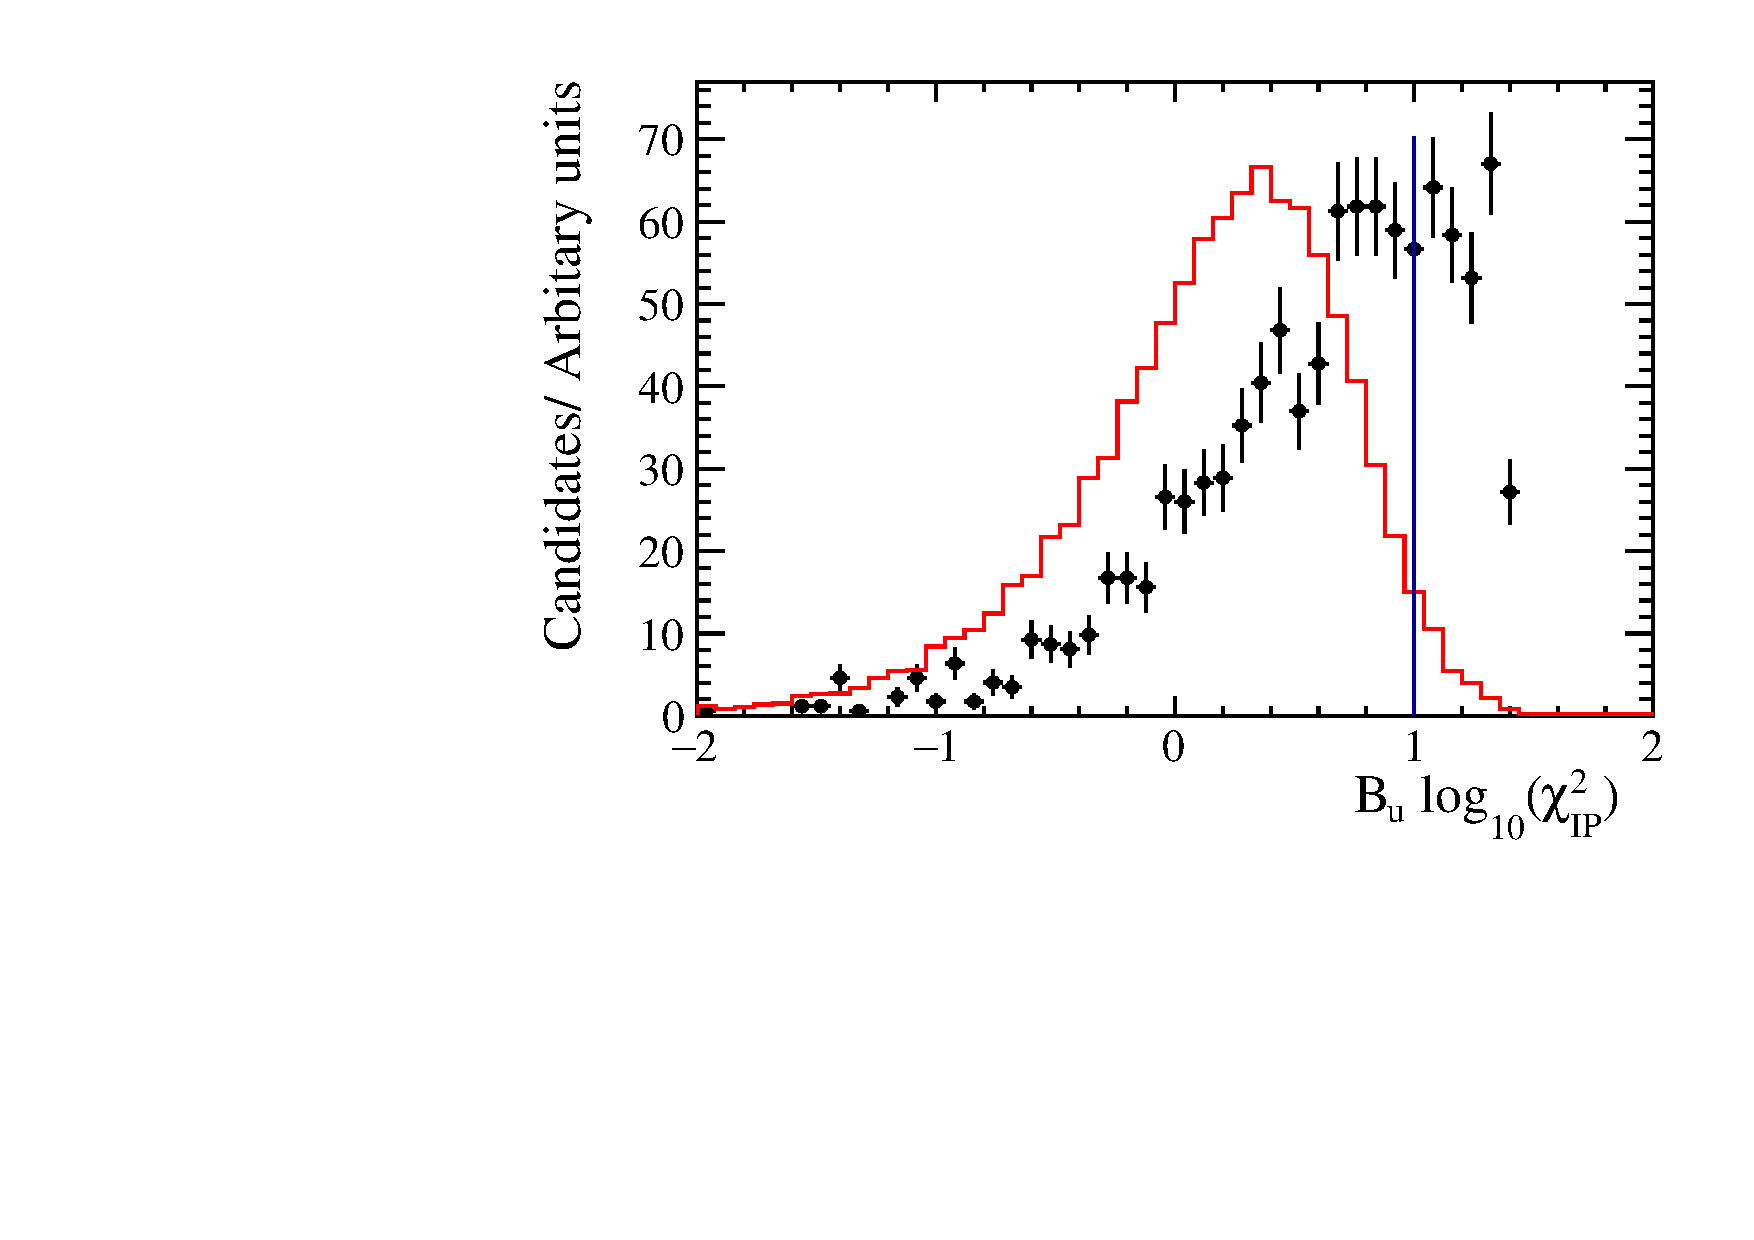
\includegraphics[width=1.0\textwidth]{figs/Selection/Data_MC_Comparison_Var_1_B2DsPhi_Ds2KKPi.pdf}
      \caption{\decay{\Dsp}{\Kp\Km\pip}}
   \end{subfigure}
   \begin{subfigure}[t]{0.32\textwidth}
      \centering
      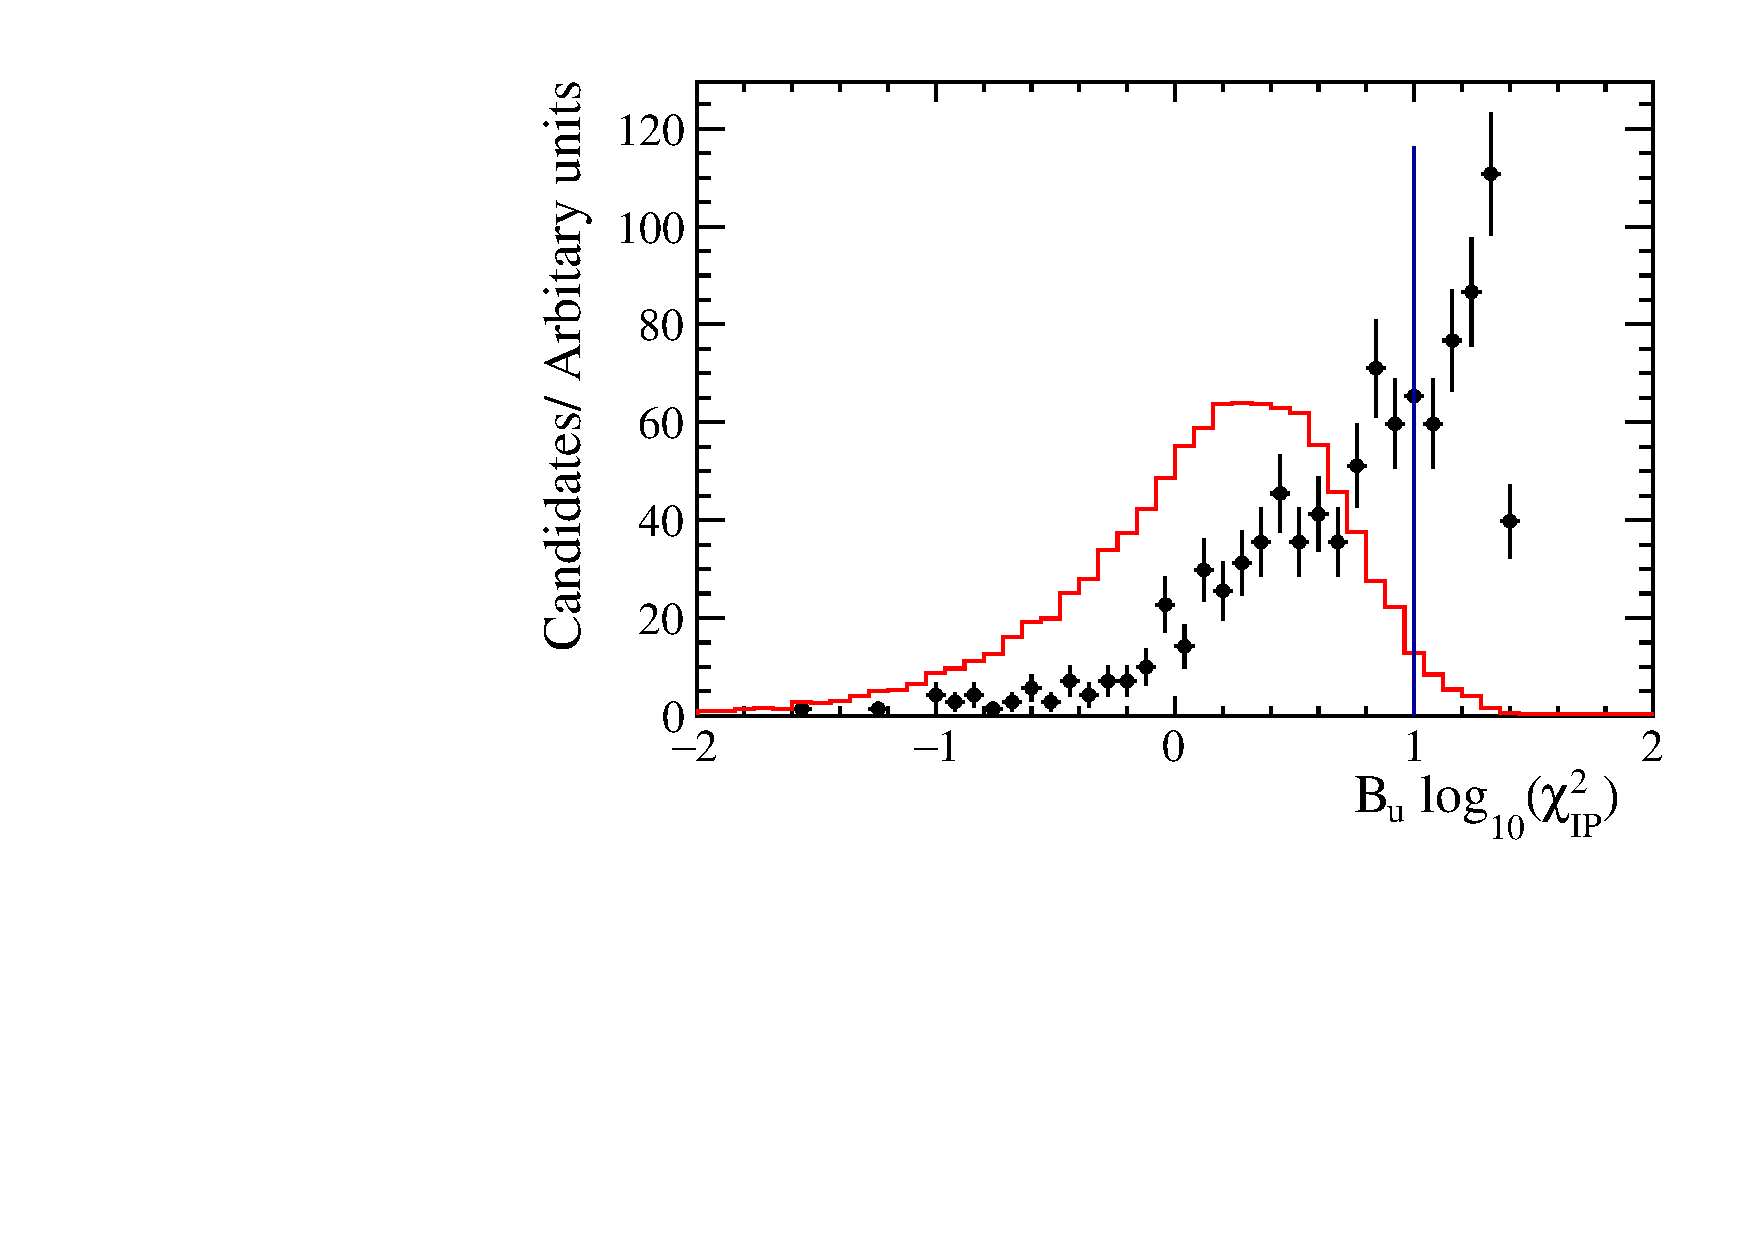
\includegraphics[width=1.0\textwidth]{figs/Selection/Data_MC_Comparison_Var_1_B2DsPhi_Ds2PiPiPi.pdf}
      \caption{\decay{\Dsp}{\pip\pim\pip}}
   \end{subfigure}
   \begin{subfigure}[t]{0.32\textwidth}
      \centering
      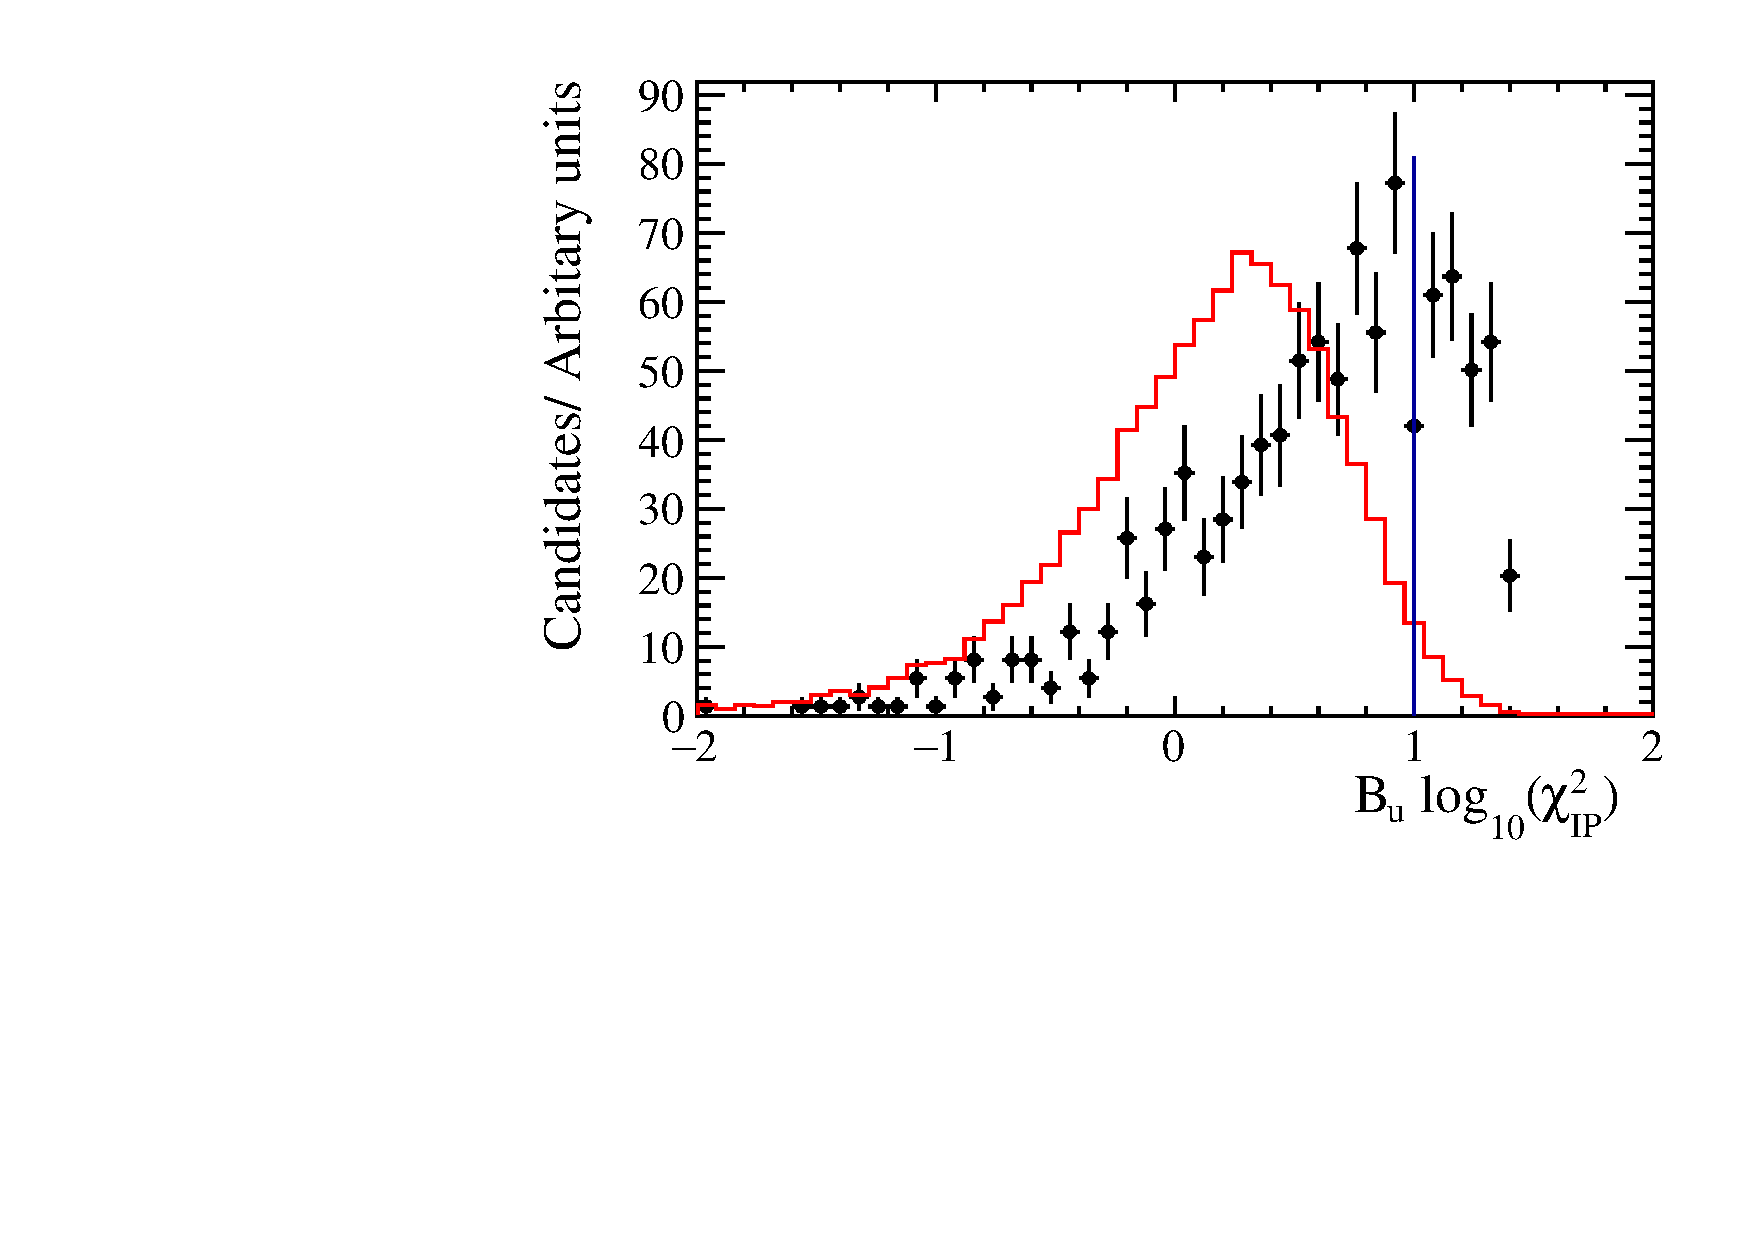
\includegraphics[width=1.0\textwidth]{figs/Selection/Data_MC_Comparison_Var_1_B2DsPhi_Ds2KPiPi.pdf}
      \caption{\decay{\Dsp}{\Kp\pim\pip}}
   \end{subfigure}\\
   \caption{The \Dsp meson $\chi^{2}_{\text{IP}}$ distributions for \decay{\Bp}{\Dsp\phiz} candidates in data (black) and simulation (red) after the MVA selection. Candidates within the range $4900 < m(\Dsp\phiz) < 5900 \mevcc$ are included in these figures. Candidates to the right of the vertical line are retained.}
   \label{fig:ipchi2dist_signal_D}   
\end{figure}
%%%%%%%%%%%%%%%%%%%%%%%%%%%%%%%%%%%%%%%%%%%%%%%%%%%%%%%%%%

The distributions for the \Bp and \Dsp meson impact parameter significance is shown in Figs.~\ref{fig:ipchi2dist_signal_B} and~\ref{fig:ipchi2dist_signal_D} respectively for \decay{\Bp}{\Dsp\phiz} candidates. The requirement values are represented by vertical lines. Small peaks can be observed at low \Dsp meson impact parameter significance, corresponding to \Dsp mesons that originated at the PV. 
As a cross-check, the same distributions are produced for the normalisation channel, \decay{\Bp}{\Dsp\Dzb}. 
As there are plentiful numbers of events, only those within $20\mevcc$ of the \Bp mass are included. The normalisation sample has a very high purity so this effectively isolates these decays in data. This comparison of data and simulation distributions is shown in Fig.~\ref{fig:ipchi2dist_normalisation}.

%%%%%%%%%%%%%%%%%%%%%%%%%%%%%%%%%%%%%%%%%%%%%%%%%%%%%%%%%%
\begin{figure}[!h]
   \centering
   \begin{subfigure}[t]{0.32\textwidth}
      \centering
      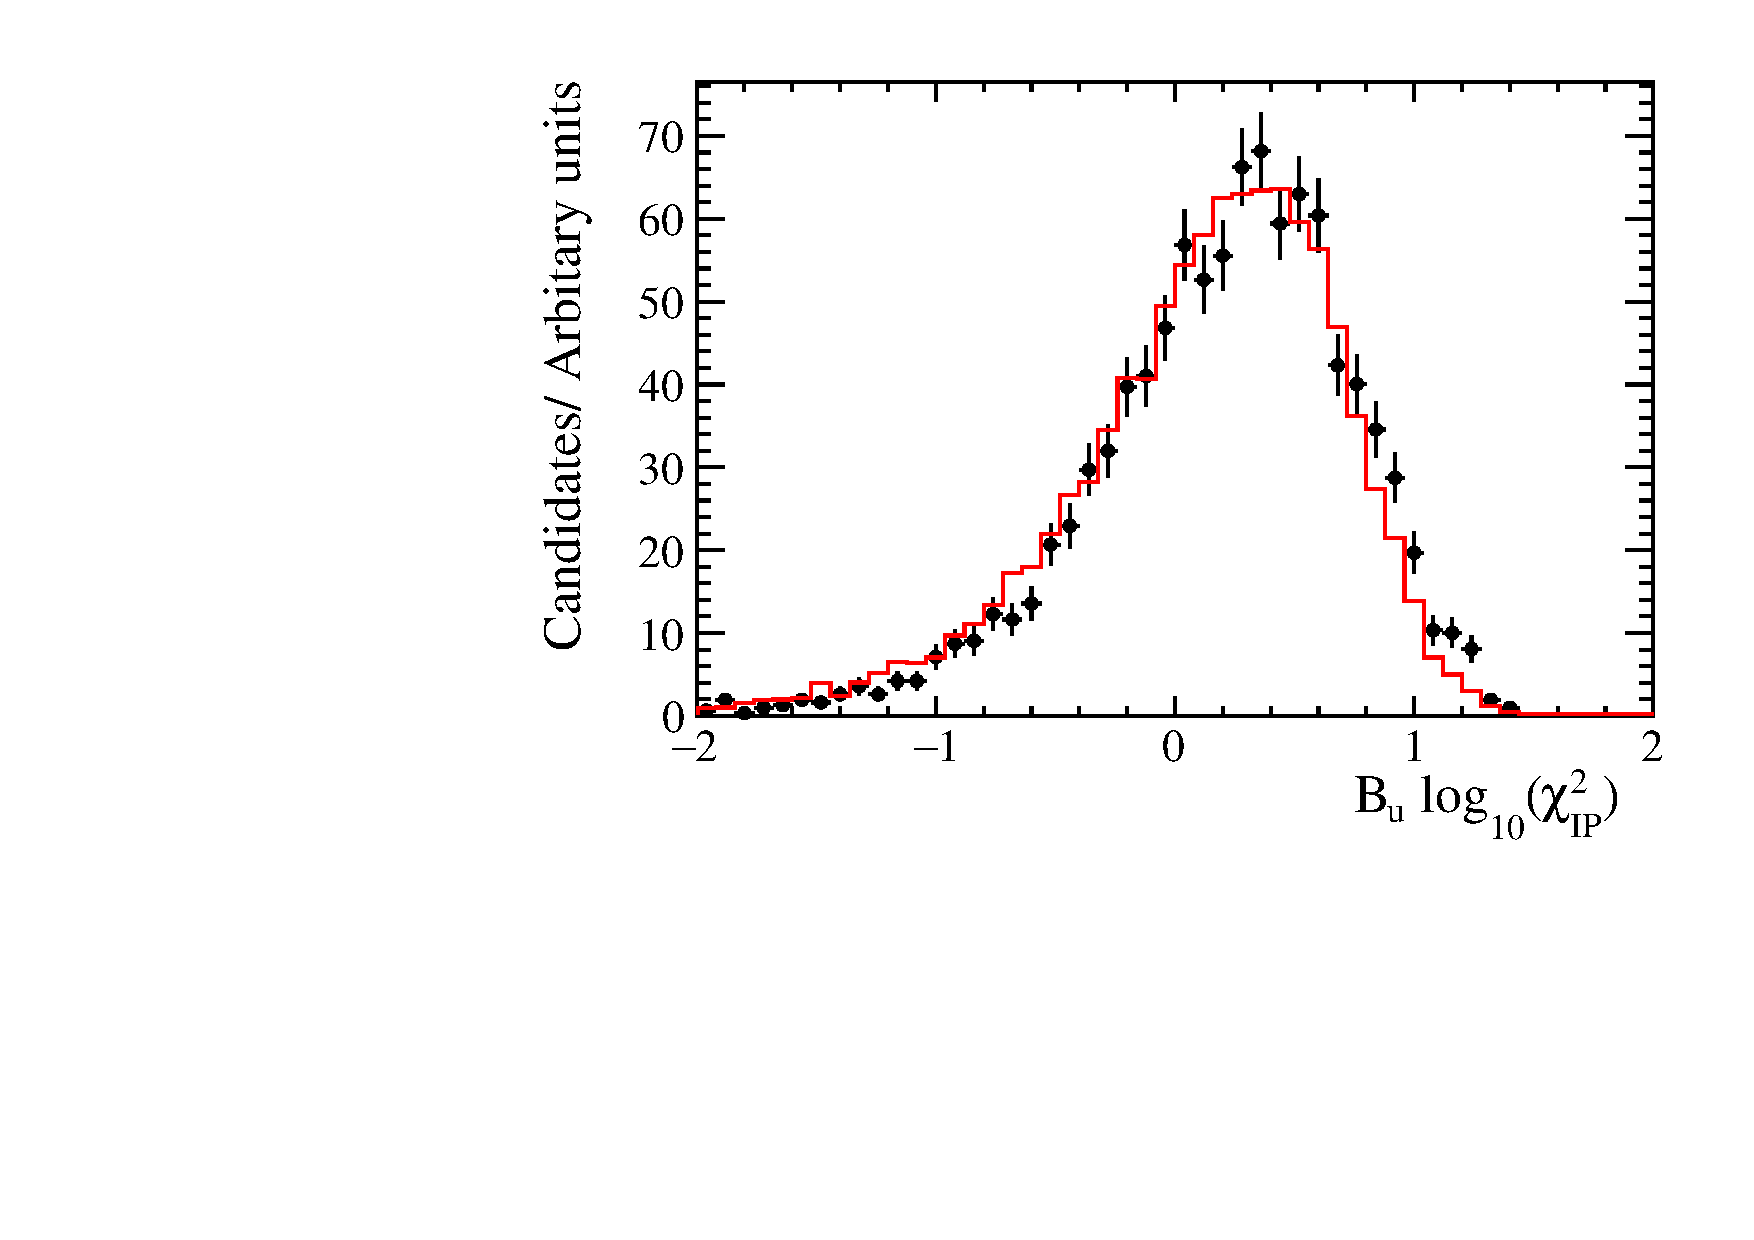
\includegraphics[width=1.0\textwidth]{figs/Selection/Data_MC_Comparison_Var_1_B2DsD0_Ds2KKPi.pdf}
      \caption{\decay{\Dsp}{\Kp\Km\pip}}
   \end{subfigure}
   \begin{subfigure}[t]{0.32\textwidth}
      \centering
      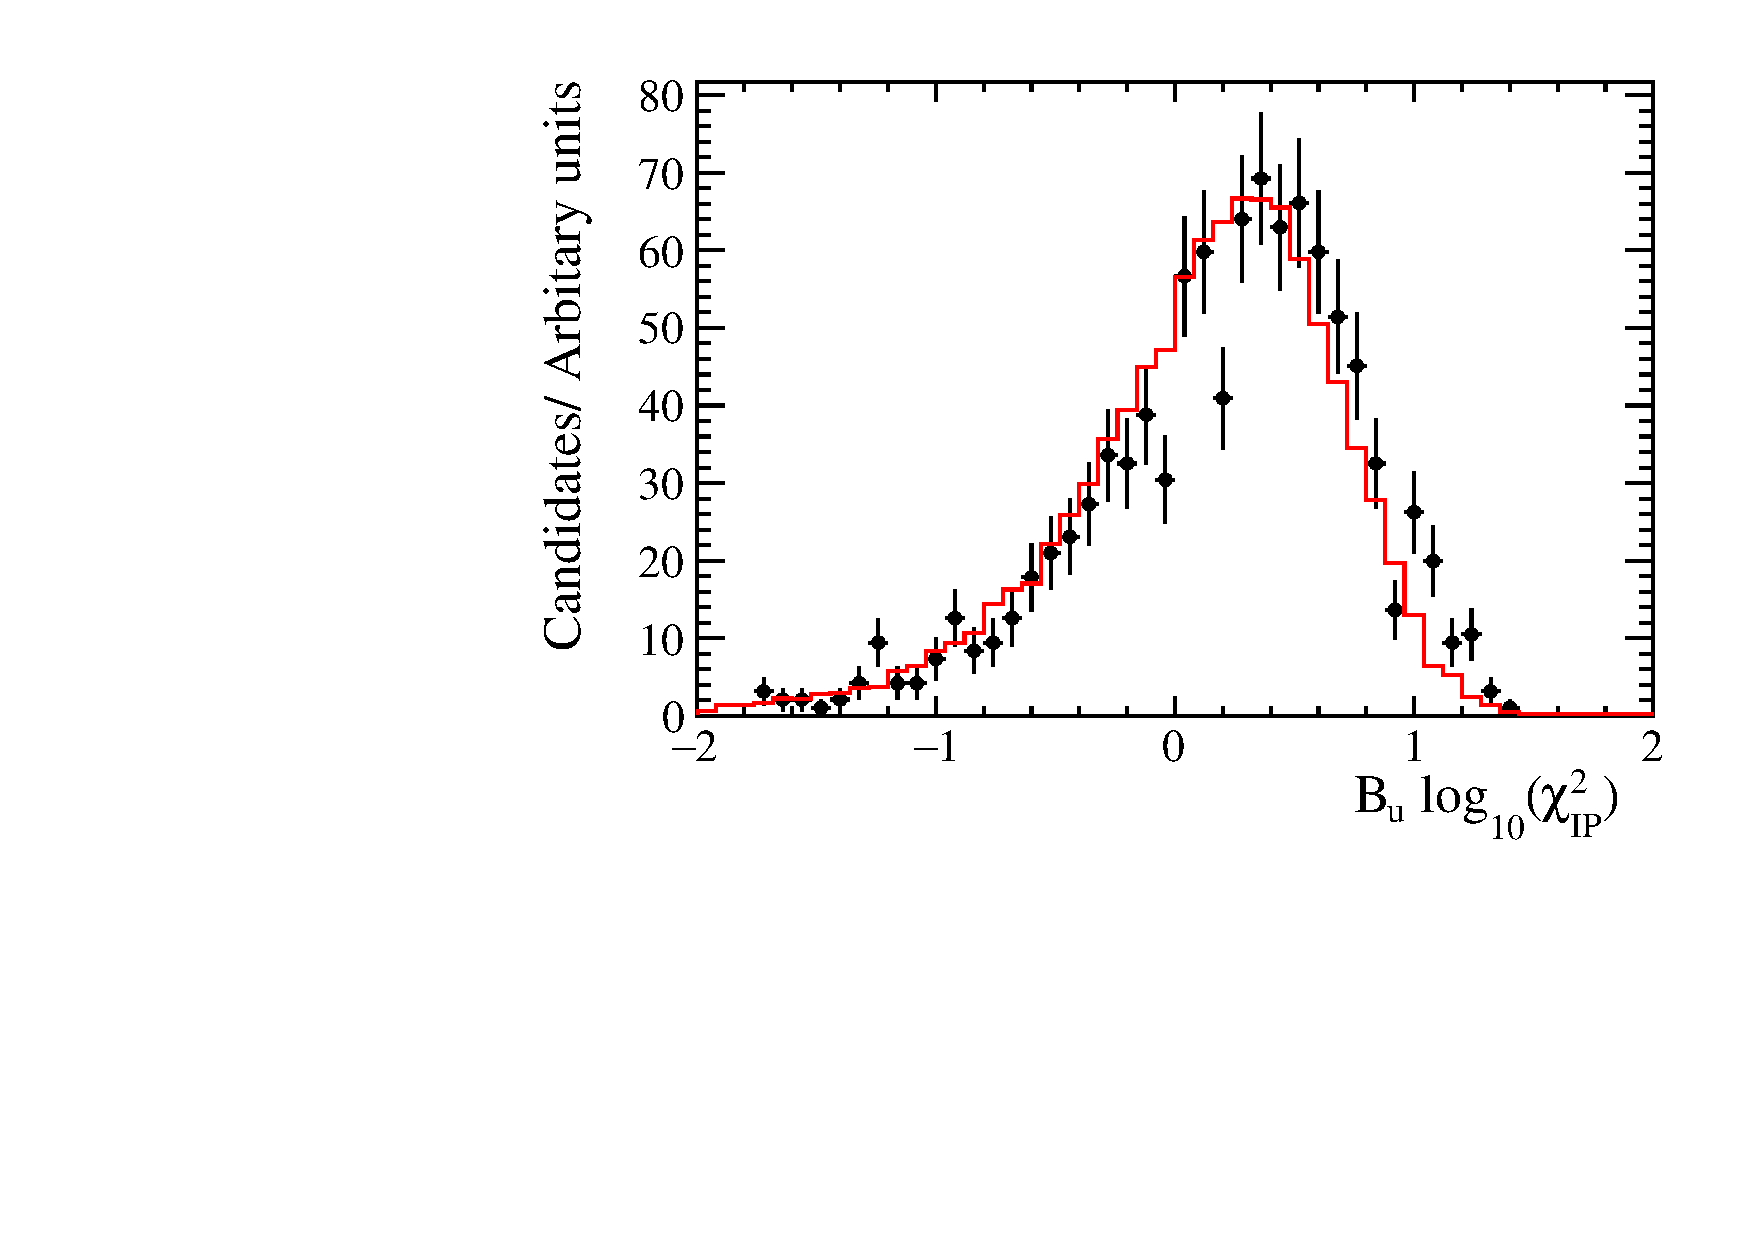
\includegraphics[width=1.0\textwidth]{figs/Selection/Data_MC_Comparison_Var_1_B2DsD0_Ds2PiPiPi.pdf}
      \caption{\decay{\Dsp}{\pip\pim\pip}}
   \end{subfigure}
   \begin{subfigure}[t]{0.32\textwidth}
      \centering
      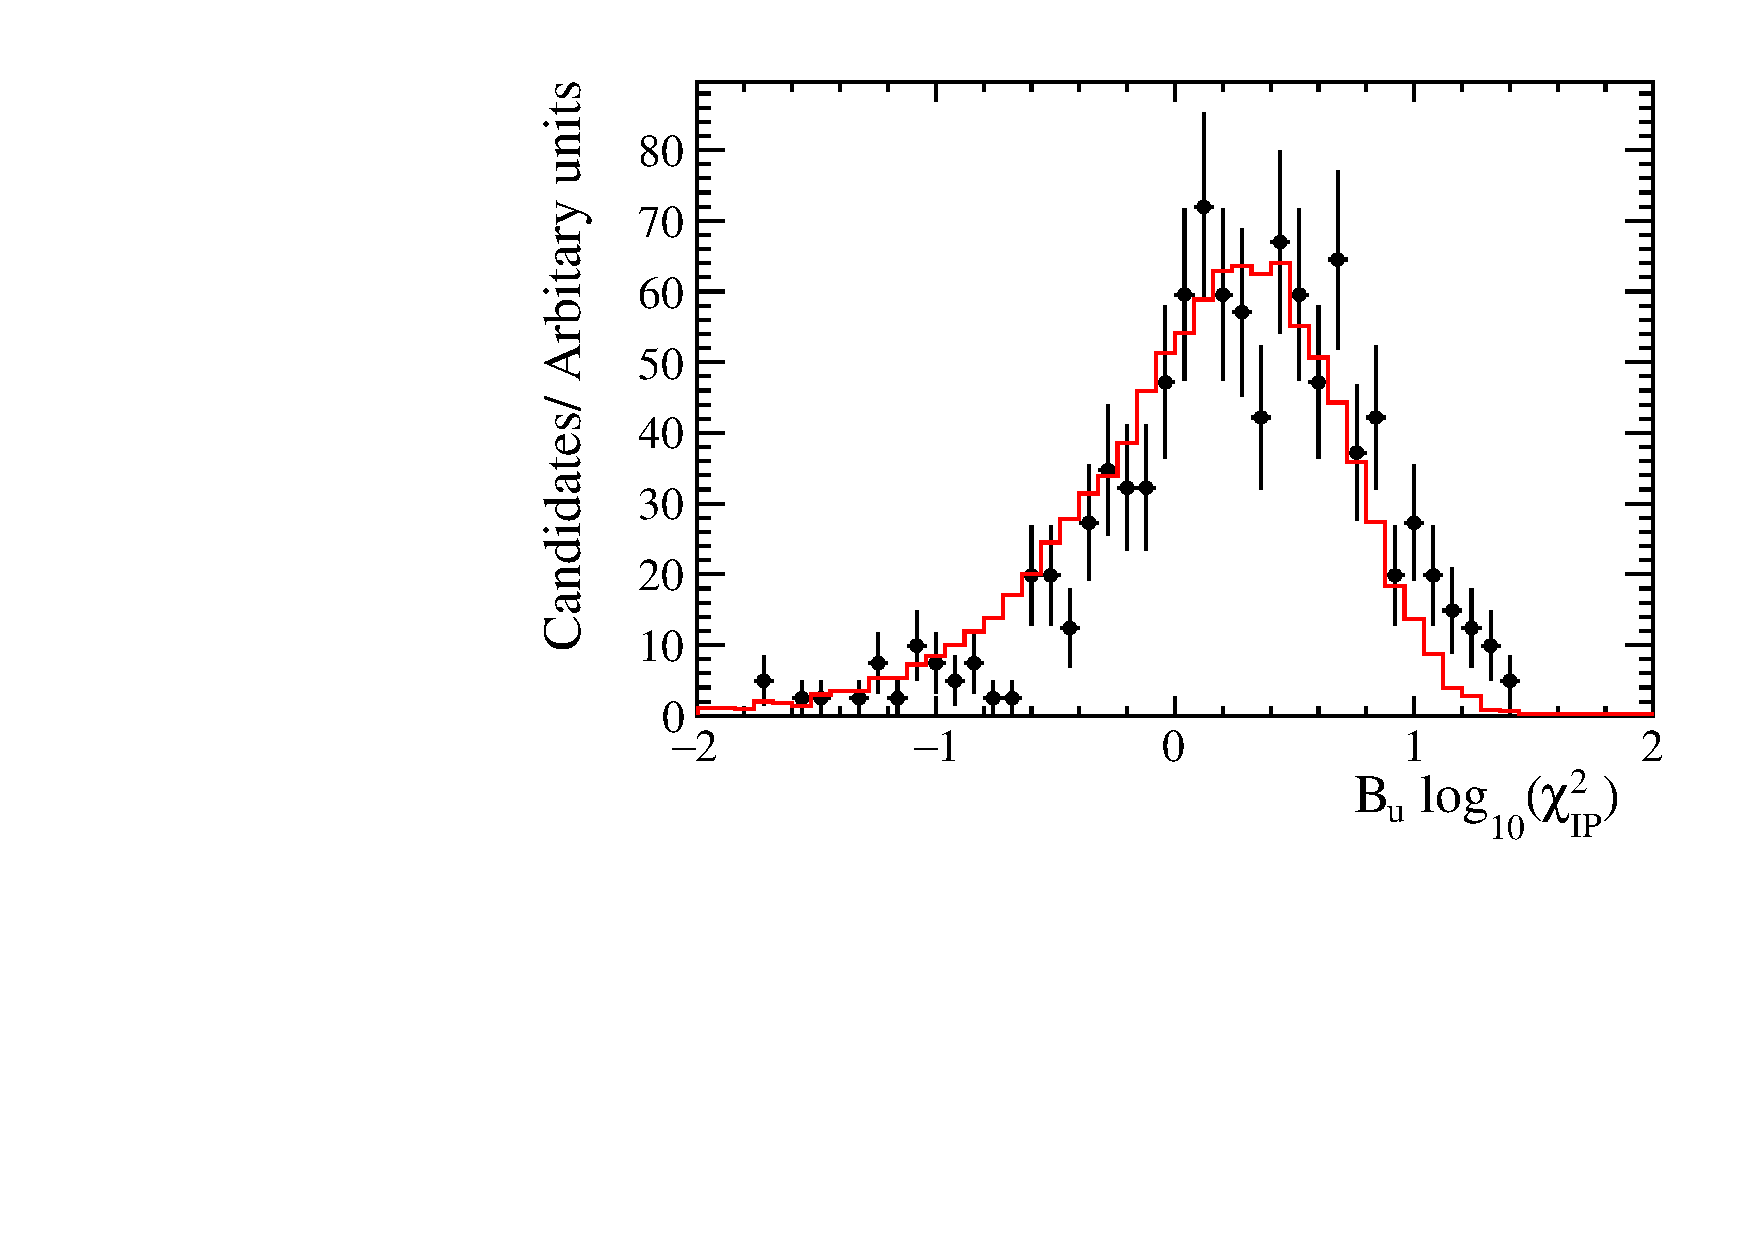
\includegraphics[width=1.0\textwidth]{figs/Selection/Data_MC_Comparison_Var_1_B2DsD0_Ds2KPiPi.pdf}
      \caption{\decay{\Dsp}{\Kp\pim\pip}}
   \end{subfigure}\\
   \begin{subfigure}[t]{0.32\textwidth}
      \centering
      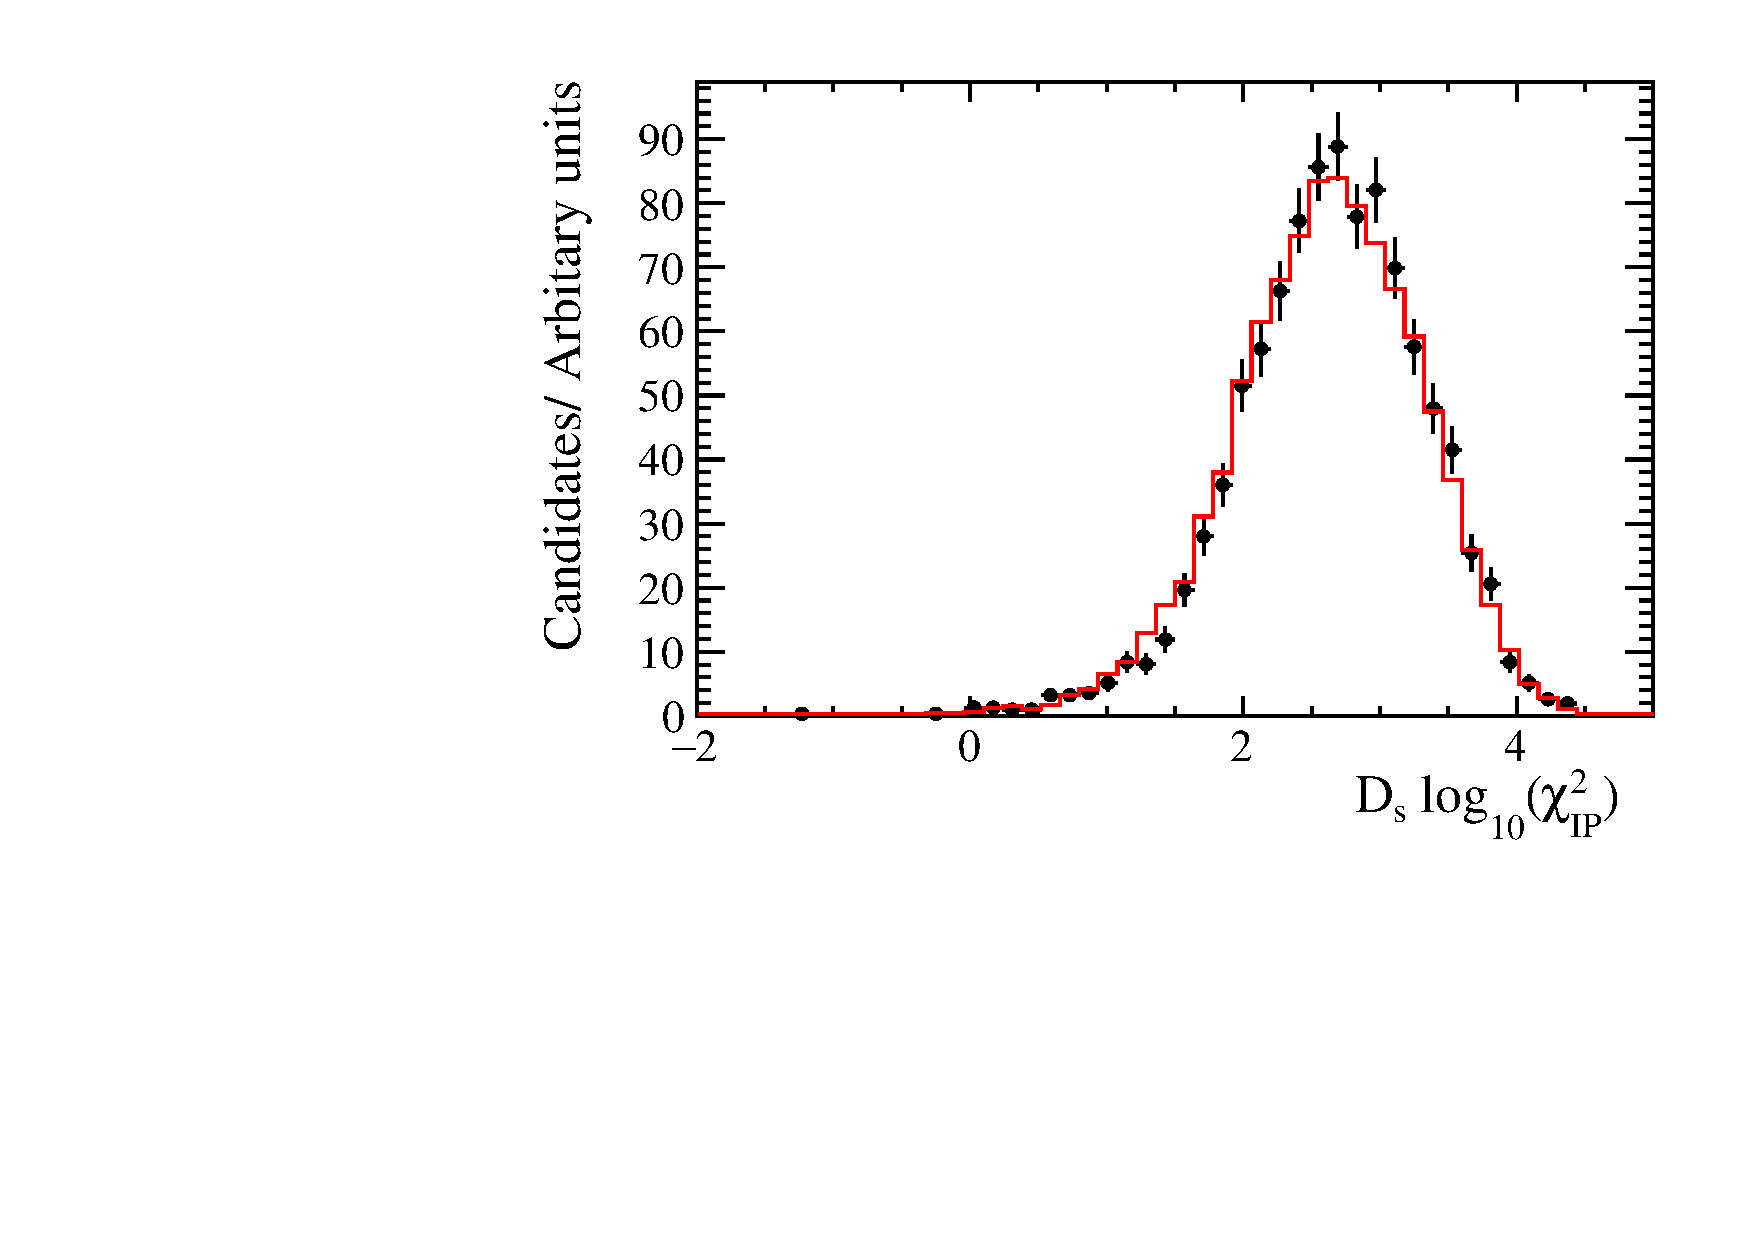
\includegraphics[width=1.0\textwidth]{figs/Selection/Data_MC_Comparison_Var_2_B2DsD0_Ds2KKPi.pdf}
      \caption{\decay{\Dsp}{\Kp\Km\pip}}
   \end{subfigure}
   \begin{subfigure}[t]{0.32\textwidth}
      \centering
      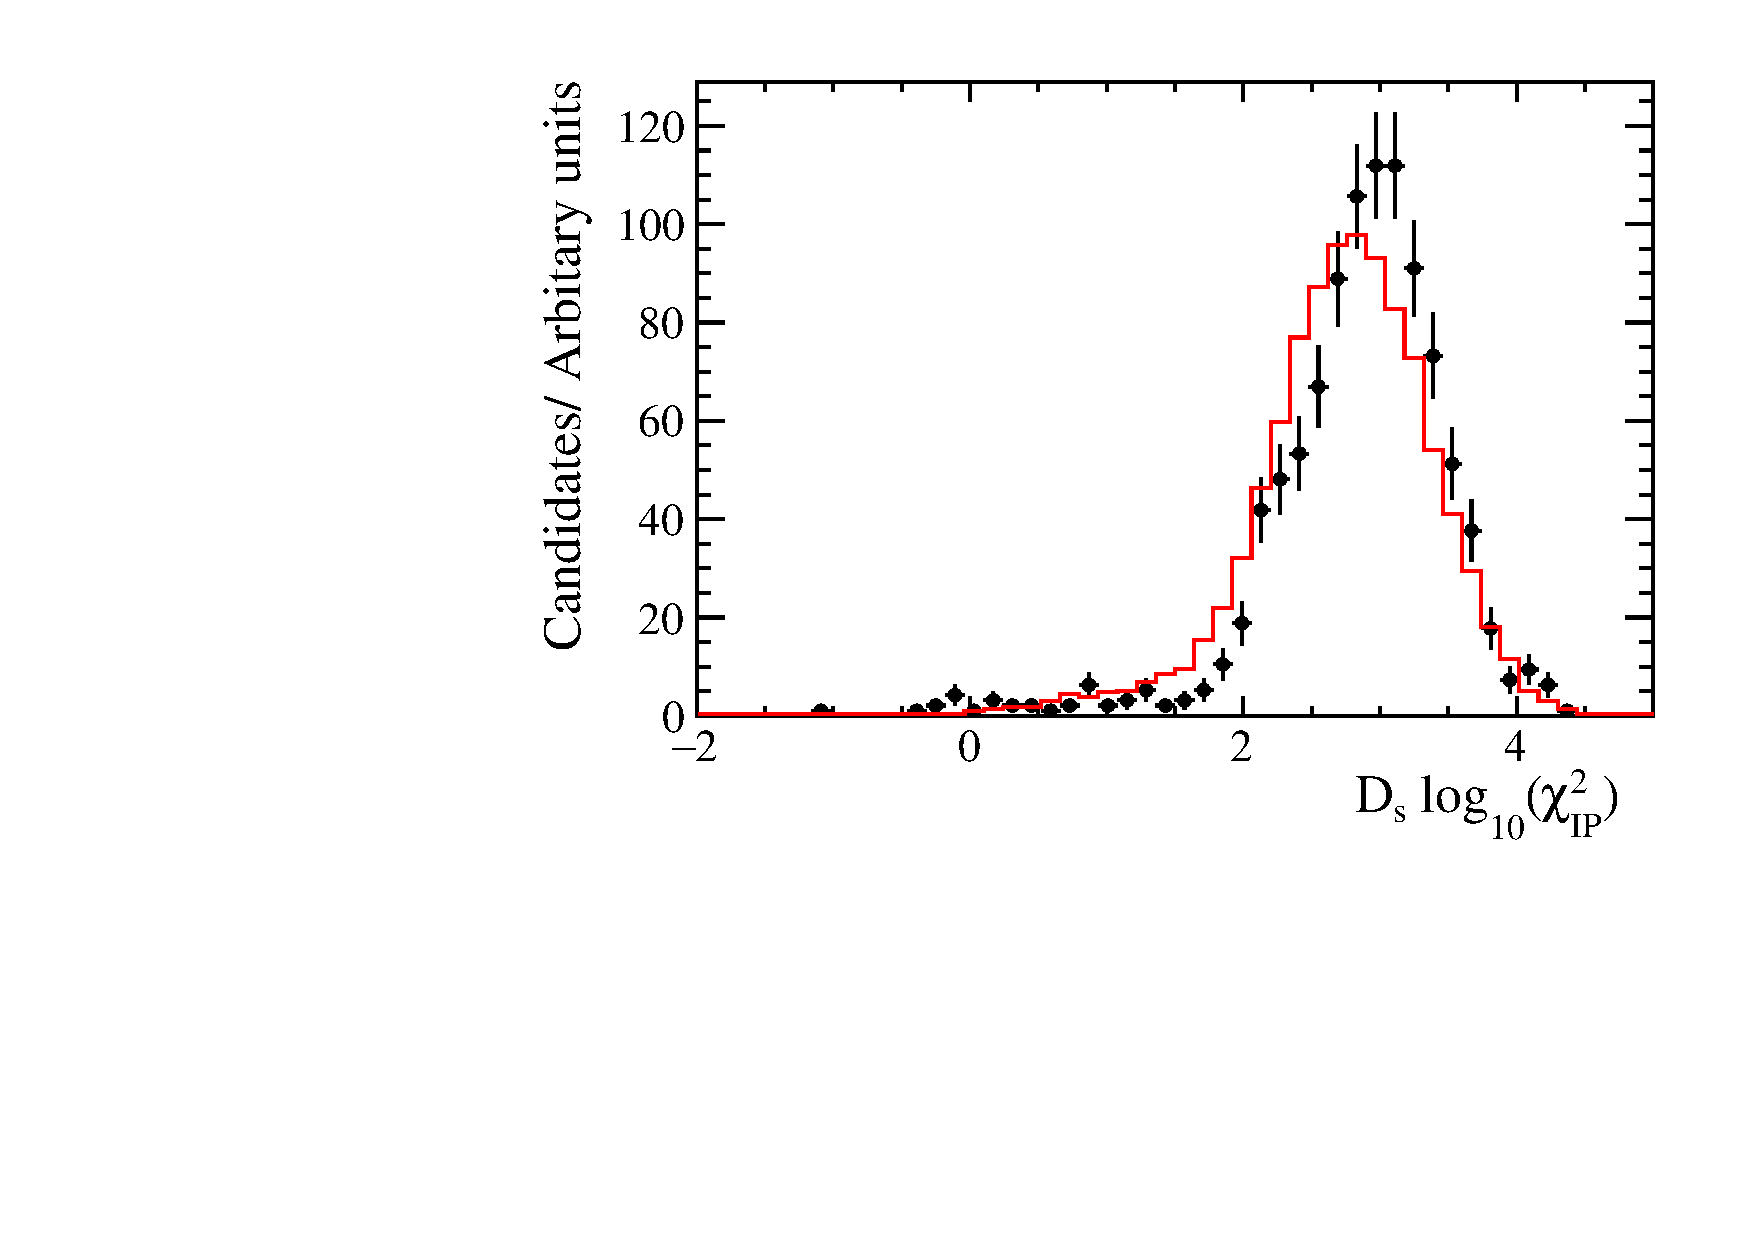
\includegraphics[width=1.0\textwidth]{figs/Selection/Data_MC_Comparison_Var_2_B2DsD0_Ds2PiPiPi.pdf}
      \caption{\decay{\Dsp}{\pip\pim\pip}}
   \end{subfigure}
   \begin{subfigure}[t]{0.32\textwidth}
      \centering
      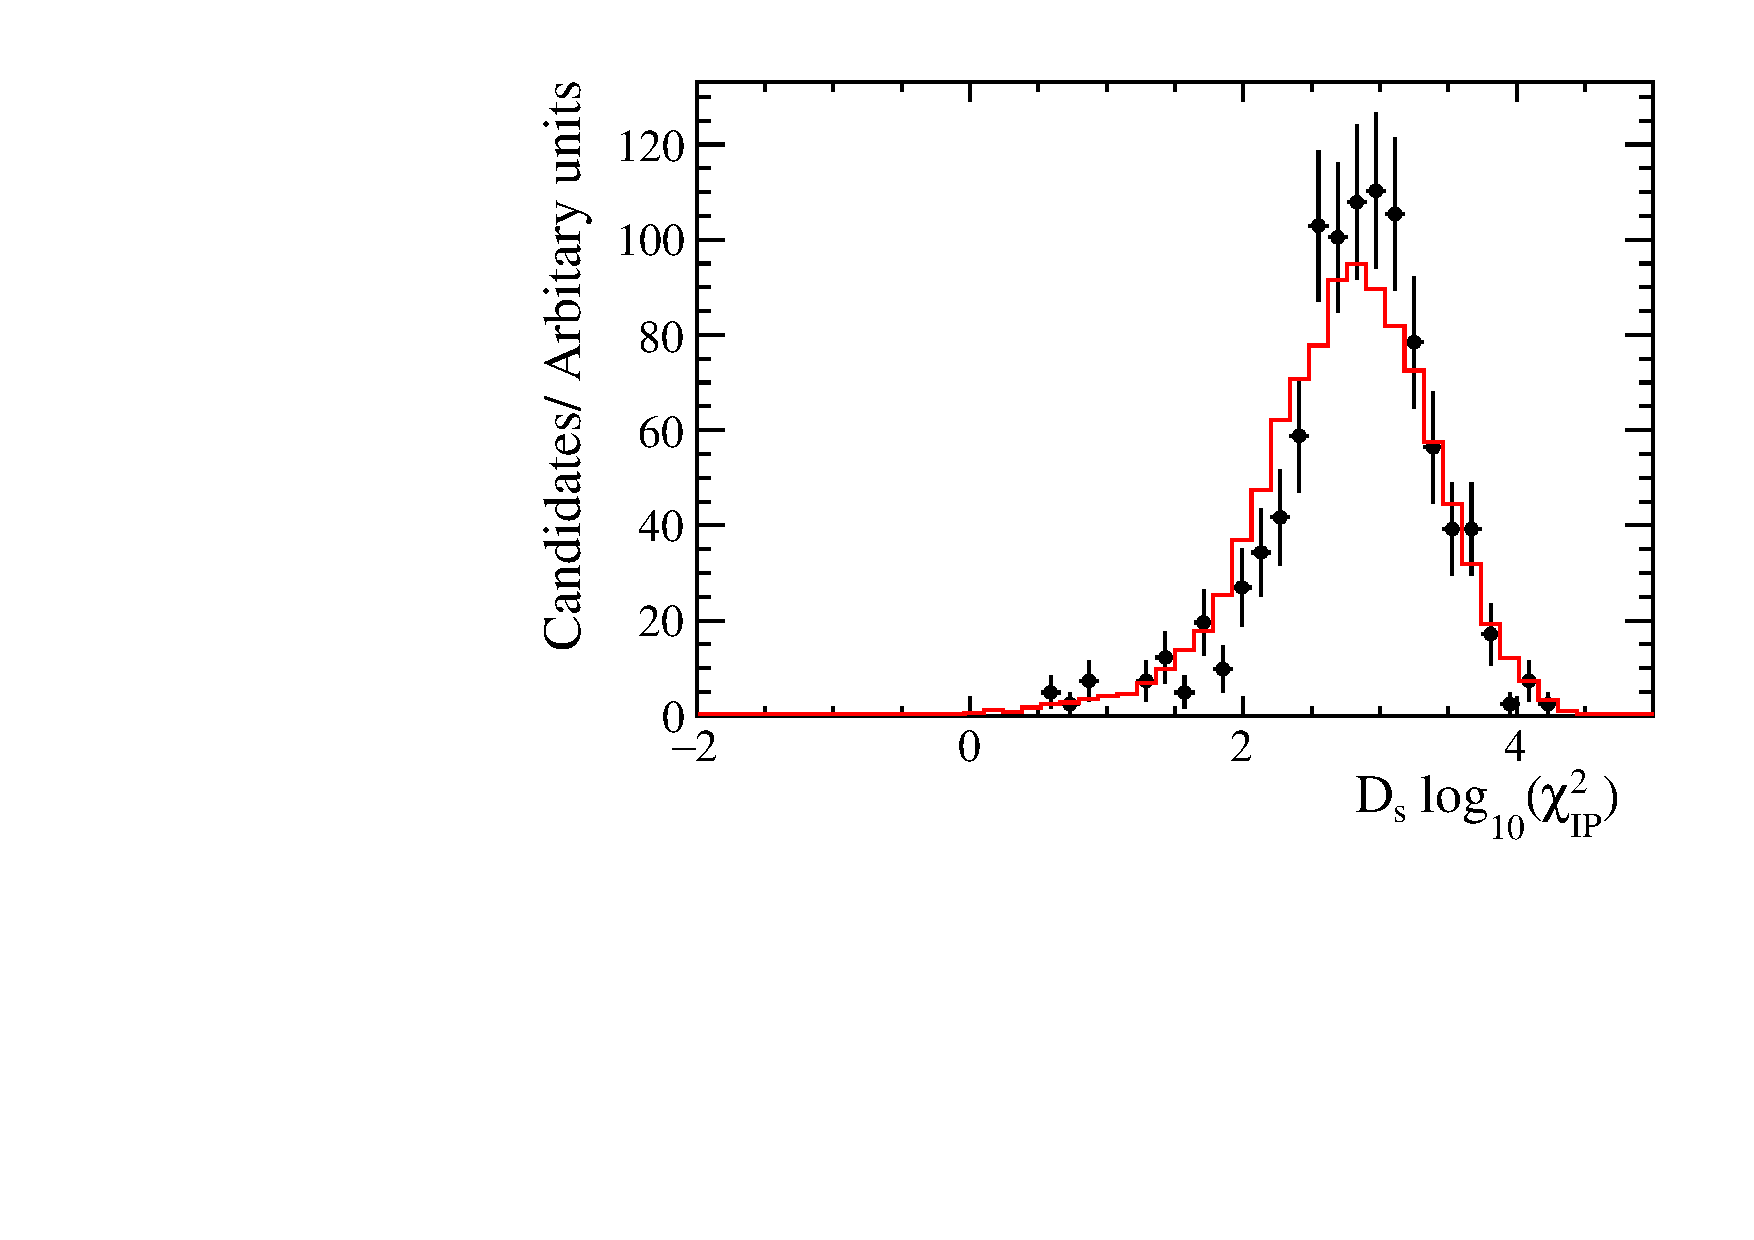
\includegraphics[width=1.0\textwidth]{figs/Selection/Data_MC_Comparison_Var_2_B2DsD0_Ds2KPiPi.pdf}
      \caption{\decay{\Dsp}{\Kp\pim\pip}}
   \end{subfigure}\\
   \caption{The \Bp and \Dsp meson $\chi^{2}_{\text{IP}}$ distributions for \decay{\Bp}{\Dsp\Dzb} candidates in data (black) and simulation (red). Candidates within the range $|m(\Dsp\phiz) - m(\Bp)| < 20 \mevcc$ are included in these figures, effectively isolating the normalisation events in data.}
   \label{fig:ipchi2dist_normalisation}   
\end{figure}
%%%%%%%%%%%%%%%%%%%%%%%%%%%%%%%%%%%%%%%%%%%%%%%%%%%%%%%%%%



Small shifts are observed in the $\chi^{2}_{\text{IP}}$ distributions. These differences are studied as a source of systematic uncertainty as discussed in Sections~\ref{sec:B2DsKK_systuncertainy} and \ref{sec:B2DsPhi_systuncertainy}.


